\documentclass[12pt]{beamer}
\usepackage{../Estilos/BeamerMAF}
\usepackage{../Estilos/ColoresLatex}
\usetheme{Warsaw}
\usecolortheme{seahorse}
%\useoutertheme{default}
\setbeamercovered{invisible}
% or whatever (possibly just delete it)
\setbeamertemplate{section in toc}[sections numbered]
\setbeamertemplate{subsection in toc}[subsections numbered]
\setbeamertemplate{subsection in toc}{\leavevmode\leftskip=3.2em\rlap{\hskip-2em\inserttocsectionnumber.\inserttocsubsectionnumber}\inserttocsubsection\par}
\setbeamercolor{section in toc}{fg=blue}
\setbeamercolor{subsection in toc}{fg=blue}
\setbeamercolor{frametitle}{fg=blue}
\setbeamertemplate{caption}[numbered]

\setbeamertemplate{footline}
\beamertemplatenavigationsymbolsempty
\setbeamertemplate{headline}{}


\makeatletter
\setbeamercolor{section in foot}{bg=gray!30, fg=black!90!orange}
\setbeamercolor{subsection in foot}{bg=blue!30}
\setbeamercolor{date in foot}{bg=black}
\setbeamertemplate{footline}
{
  \leavevmode%
  \hbox{%
  \begin{beamercolorbox}[wd=.333333\paperwidth,ht=2.25ex,dp=1ex,center]{section in foot}%
    \usebeamerfont{section in foot} \insertsection
  \end{beamercolorbox}%
  \begin{beamercolorbox}[wd=.333333\paperwidth,ht=2.25ex,dp=1ex,center]{subsection in foot}%
    \usebeamerfont{subsection in foot}  \insertsubsection
  \end{beamercolorbox}%
  \begin{beamercolorbox}[wd=.333333\paperwidth,ht=2.25ex,dp=1ex,right]{date in head/foot}%
    \usebeamerfont{date in head/foot} \insertshortdate{} \hspace*{2em}
    \insertframenumber{} / \inserttotalframenumber \hspace*{2ex} 
  \end{beamercolorbox}}%
  \vskip0pt%
}
\makeatother

\makeatletter
\patchcmd{\beamer@sectionintoc}{\vskip1.5em}{\vskip0.8em}{}{}
\makeatother

\newlength{\depthofsumsign}
\setlength{\depthofsumsign}{\depthof{$\sum$}}
\newcommand{\nsum}[1][1.4]{% only for \displaystyle
    \mathop{%
        \raisebox
            {-#1\depthofsumsign+1\depthofsumsign}
            {\scalebox
                {#1}
                {$\displaystyle\sum$}%
            }
    }
}
\def\scaleint#1{\vcenter{\hbox{\scaleto[3ex]{\displaystyle\int}{#1}}}}
\def\scaleoint#1{\vcenter{\hbox{\scaleto[3ex]{\displaystyle\oint}{#1}}}}
\def\bs{\mkern-12mu}


\AtBeginDocument{\RenewCommandCopy\qty\SI}
\ExplSyntaxOn
\msg_redirect_name:nnn { siunitx } { physics-pkg } { none }
\ExplSyntaxOff

\title{\large{3 - Construcción de sistemas coord. especiales}}
\subtitle{Tema 1 - La física y la geometría}

\author{M. en C. Gustavo Contreras Mayén}
\makeatletter

\setbeamertemplate{footline}
{
  \leavevmode%
  \hbox{%
  \begin{beamercolorbox}[wd=.333333\paperwidth,ht=2.25ex,dp=1ex,center]{section in foot}%
    \usebeamerfont{section in foot} \insertsection
  \end{beamercolorbox}%
  \begin{beamercolorbox}[wd=.333333\paperwidth,ht=2.25ex,dp=1ex,center]{subsection in foot}%
    \usebeamerfont{subsection in foot}  \insertsubsection
  \end{beamercolorbox}%
  \begin{beamercolorbox}[wd=.333333\paperwidth,ht=2.25ex,dp=1ex,right]{date in head/foot}%
    \usebeamerfont{date in head/foot} {T1 - Tercera presentación} \hspace*{2em}
    \insertframenumber{} / \inserttotalframenumber \hspace*{2ex} 
  \end{beamercolorbox}}%
  \vskip0pt%
}
\makeatother
\date{}

\begin{document}
\maketitle
\fontsize{14}{14}\selectfont
\spanishdecimal{.}

\section*{Contenido}
\frame[allowframebreaks]{\frametitle{Contenido} \tableofcontents[currentsection, hideallsubsections]}

\section{Construcción de sistemas coordenados}
\frame[allowframebreaks]{\frametitle{Temas a revisar} \tableofcontents[currentsection, hideothersubsections]}
\subsection{Introducción}

\begin{frame}
\frametitle{Introducción}
Una pregunta importante que planteamos en este momento es: ¿para qué estamos revisando los sistemas coordenados curvilíneos?
\\
\bigskip
\pause
Como respuesta presentamos la siguiente:
\end{frame}
\begin{frame}
\frametitle{Introducción}
Ante un problema de la física, debemos de seleccionar el sistema coordenado de modo que se adapte al problema, \textocolor{ao(english)}{para aprovechar cualquier oportunidad o simetría presente en el mismo}.
\\
\bigskip
\pause
De tal manera que resultará más fácil la solución que cuando se obliga a adaptar una solución en un sistema cartesiano.
\end{frame}
\begin{frame}
\frametitle{Introducción}
Cuando se menciona que \enquote{es más fácil la solución}, significa que se tendrá una ecuación diferencial parcial (EDP) que pueda separarse en ecuaciones diferenciales ordinarias (EDO), frecuentemente en la \enquote{forma estándar} en el nuevo sistema coordenado.
\\
\bigskip
\pause
La \textocolor{amethyst}{técnica de separación de variables}, se verá en el Tema 2 del curso.
\end{frame}

\subsection{Sistemas coordenados especiales}

\begin{frame}
\frametitle{Otros sistemas coordenados}
Conocemos al menos tres sistemas coordenados con los que hemos trabajado en distintas áreas de nuestra carrera: cartesiano, cilíndrico (en 3D, polar en 2D) y esférico.
\\
\bigskip
\pause
De manera conveniente enlistamos catorce sistemas coordenados, que en algún momento nos podremos encontrar.
\end{frame}
\begin{frame}
\frametitle{Aviso importante}
Como punto importante debemos de señalar que no es intención de curso que se haga una revisión completa, detallada para cada uno de los sistemas.
\end{frame}
\begin{frame}
\frametitle{Aviso importante}
Más bien, veremos una metodología con la cual abordaremos el estudio de un sistema coordenado, y entonces tendremos la manera de estudiar otros de acuerdo a las necesidades que se nos presenten.
\end{frame}
\begin{frame}
\frametitle{Otros sistemas coordenados}
De manera conveniente se presenta una lista con catorce sistemas, clasificando los mismos de acuerdo con el hecho de que tengan o no:
\setbeamercolor{item projected}{bg=aureolin,fg=auburn}
\setbeamertemplate{enumerate items}{%
\usebeamercolor[bg]{item projected}%
\raisebox{1.5pt}{\colorbox{bg}{\color{fg}\footnotesize\insertenumlabel}}%
}
\begin{enumerate}[<+->]
\item Un eje de traslación (perpendicular a la familia de superficies de plano paralelo)
\item Un eje de simetría rotacional.
\end{enumerate}
\end{frame}
\begin{frame}
\frametitle{Sistemas coordenados especiales}
\fontsize{8}{8}\selectfont
{
\renewcommand{\arraystretch}{1.2}
\begin{table}[H]
\centering
\begin{tabular}{p{3cm} p{4cm} p{2.5cm}}
Eje de traslación & Eje de rotación & Ninguno \\ \hline
Cartesiano ($3$ ejes) & & Confocal elipsoidal \\
Circular cilíndrico & Circular cilíndrico & \\
& Polar esferoidal ($3$ ejes) & \\
Elíptico cilíndrico & Esferoidal prolato o alargado & \\
& Esferoidal oblato & \\
Parabólico cilíndrico & Parabólico & \\
Bipolar & Toroidal & \\
& Biesférico & \\[0.5em]
& & Cónico \\
& & Confocal paraboidal \\
\end{tabular}
\end{table}
}
\end{frame}
% \begin{frame}
% \frametitle{Sistemas coordenados especiales}
% El espaciamiento en la tabla indica las relaciones entre los diversos sistemas coordenados.
% \\
% \bigskip
% \pause
% Si se considera el caso en dos dimensiones ($z = 0$) de un sistema con un eje de traslación (columna izquierda) y se le hace girar alrededor de un eje de simetría de reflexión, se genera el sistema coordenado correspondiente indicado en la columna central hacia la derecha.
% \end{frame}
% \begin{frame}
% \frametitle{Sistemas coordenados especiales}
% Por ejemplo: la rotación del plano $z = 0$ del sistema cilíndrico elíptico alrededor del eje principal genera el sistema esferoidal alargado; la rotación alrededor del eje menor resulta en el sistema esferoidal oblato.
% \end{frame}
% \begin{frame}
% \frametitle{Sistemas coordenados especiales}
% También se consideran tres sistemas que no tienen eje de traslación o eje de rotación.
% \\
% \bigskip
% \pause
% En este grupo asimétrico, el sistema elipsoidal confocal se utiliza algunas veces como el sistema más general y del que casi todos los demás sistemas se obtienen del mismo.
% \end{frame}

\section{Desarrollo de un sistema coordenado 1/2}
\frame[allowframebreaks]{\frametitle{Temas a revisar} \tableofcontents[currentsection, hideothersubsections]}
\subsection{Coord. cilíndricas elípticas \texorpdfstring{$(u, v, z)$}{(u, v, z)}.}

\begin{frame}
\frametitle{Desarrollo para un sistema especial}
A continuación veremos la manera de abordar un sistema coordenado especial, para determinar:
\pause
\setbeamercolor{item projected}{bg=cadetblue,fg=white}
\setbeamertemplate{enumerate items}{%
\usebeamercolor[bg]{item projected}%
\raisebox{1.5pt}{\colorbox{bg}{\color{fg}\footnotesize\insertenumlabel}}%
}
\begin{enumerate}[<+->]
\item Las superficies constantes.
\item Los factores de escala.
\item Los operadores diferenciales.
\end{enumerate}
\pause
que serán necesarios para resolver un problema con esta geometría en particular.
\end{frame}

\subsection{Reglas de transformación}

\begin{frame}
\frametitle{Reglas de transformación - S. Cilíndrico elíptico}
Para el \textocolor{carnelian}{sistema cilíndrico elíptico}, se tienen las siguientes reglas de transformación:
\pause
\begin{eqnarray}
\begin{aligned}
(x, y, z) &\Rightarrow (u, v, z) \\[0.5em] \pause
x &= a \, \cosh u \, \cos v \\[0.5em] \pause
y &= a \, \sinh u \, \sin v \\[0.5em] \pause
z &= z
\end{aligned}
\label{eq:ecuacion_02_73_esp}
\end{eqnarray}
\end{frame}

\subsection{Superficies coordenadas}

\begin{frame}
\frametitle{Superficies coordenadas}
Para identificar las superficies constantes, elevamos al cuadrado cada lado de $x$ e $y$:
\pause
\begin{eqnarray*}
\begin{aligned}
x^{2} &= a^{2} \, \cosh^{2} u \, \cos^{2} v \label{eq:ecuacion_02_74_esp} \\[0.5em] \pause
y^{2} &= a^{2} \, \sinh^{2} u \, \sin^{2} v \label{eq:ecuacion_02_75_esp}
\end{aligned}
\end{eqnarray*}
\end{frame}
\begin{frame}
\frametitle{Superficies coordenadas}
Dividimos $x^{2}$ entre $\cos^{2} v$ \pause
\begin{eqnarray*}
\begin{aligned}
\dfrac{x^{2}}{\cos^{2} v} &= \dfrac{a^{2} \, \cosh^{2} u \, \cos^{2} v}{\cos^{2} v} \\[0.5em] \pause
\dfrac{x^{2}}{\cos^{2} v} &= a^{2} \, \cosh^{2} u \\[0.5em] \pause
\Rightarrow \hspace{0.3cm} \dfrac{x^{2}}{a^{2} \, \cosh^{2} u} &= \cos^{2} v 
\end{aligned}
\end{eqnarray*}
\end{frame}
\begin{frame}
\frametitle{Superficies coordenadas}
Luego dividimos $y^{2}$ entre $\sin^{2} v$:
\pause
\begin{eqnarray*}
\begin{aligned}
\dfrac{y^{2}}{\sin^{2} v} &= \dfrac{a^{2} \, \sinh^{2} u \, \sin^{2} v}{\sin^{2} v} = a^{2} \, \sinh^{2} u  \\[0.5em]
\Rightarrow \hspace{0.3cm} \dfrac{y^{2}}{a^{2} \, \sinh^{2} u} &= \sin^{2} v
\end{aligned}
\end{eqnarray*}
\end{frame}
\begin{frame}
\frametitle{Superficies coordenadas}
Recordamos que:
\pause
\begin{align*}
\cos^{2} v + \sin^{2} v = 1 \\[0.5em]
\cosh^{2} u - \sinh^{2} u = 1
\end{align*}
\end{frame}
\begin{frame}
\frametitle{Superficies coordenadas}
Así llegamos a:
\pause
\begin{subequations}
\begin{equation}
\dfrac{x^{2}}{a^{2} \, \cosh^{2} u} + \dfrac{y^{2}}{a^{2} \, \sinh^{2} u} = \cos^{2} v + \sin^{2} v = 1 \label{eq:ecuacion_02_76_esp}
\end{equation}
\begin{equation}
\dfrac{x^{2}}{a^{2} \, \cos^{2} v} - \dfrac{y^{2}}{a^{2} \, \sin^{2} v } = \cosh^{2} u - \sinh^{2} u = 1 \label{eq:ecuacion_02_77_esp}
\end{equation}
\end{subequations}
\end{frame}
\begin{frame}
\frametitle{Superficies coordenadas}
Para $v = $ constante, la ec. (\ref{eq:ecuacion_02_76_esp}):
\begin{align*}
\dfrac{x^{2}}{a^{2} \, \cosh^{2} u} + \dfrac{y^{2}}{a^{2} \, \sinh^{2} u} = \cos^{2} v + \sin^{2} v = 1 
\end{align*}
genera una familia de elipses con el eje $x$, en el principal.
\end{frame}
\begin{frame}
\frametitle{Superficies coordenadas}
Para $u = $ constante, la ec. (\ref{eq:ecuacion_02_77_esp})
\begin{align*}
\dfrac{x^{2}}{a^{2} \, \cos^{2} v} - \dfrac{y^{2}}{a^{2} \, \sin^{2} v } &= \cosh^{2} u - \sinh^{2} u = 1
\end{align*}
genera hipérbolas con puntos focales en el eje $x$.
\end{frame}
\begin{frame}
\frametitle{Superficies coordenadas}
\begin{figure}[H]
    \centering
    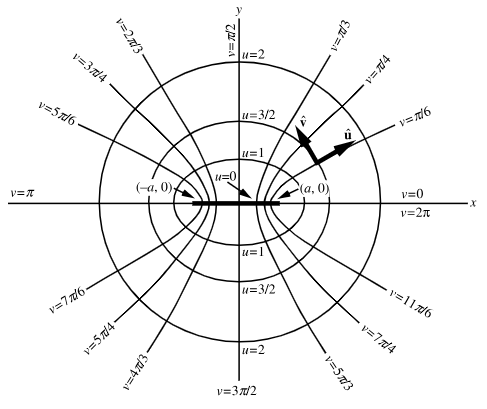
\includegraphics[scale=0.55]{Imagenes/EllipticCylindricalCoord_1000.png}
    \caption{Sistema coordenado cilíndrico elíptico en el plano $x-y$.}
    \label{fig:figura_coordenada_cilindricas_elipticas}
\end{figure}
\end{frame}
\begin{frame}
\frametitle{Superficies coordenadas}
Por último, para $z$ constante, tenemos una familia de planos en $x - y$.
\end{frame}  
\begin{frame}
\frametitle{Superficies coordenadas}
La familia de superficies coordenadas son las siguientes:
\pause
\setbeamercolor{item projected}{bg=britishracinggreen,fg=buff}
\setbeamertemplate{enumerate items}{%
\usebeamercolor[bg]{item projected}%
\raisebox{1.5pt}{\colorbox{bg}{\color{fg}\footnotesize\insertenumlabel}}%
}
\begin{enumerate}[<+->]
\item Cilindros elípticos con $u$ constante, $0 \leq u < \infty$
\item Cilindros hiperbólicos con $v$ constante, $0 \leq v \leq 2 \, \pi$
\item Planos paralelos al plano $x-y$ con $z$ constante, $-\infty < z < \infty$
\end{enumerate}
\pause
Como vemos en la siguiente figura (\ref{fig:figura_coordenada_cilindricas_elipticas_3D})
\end{frame}
\begin{frame}
\frametitle{Superficies coordenadas}
\begin{figure}[H]
    \centering
    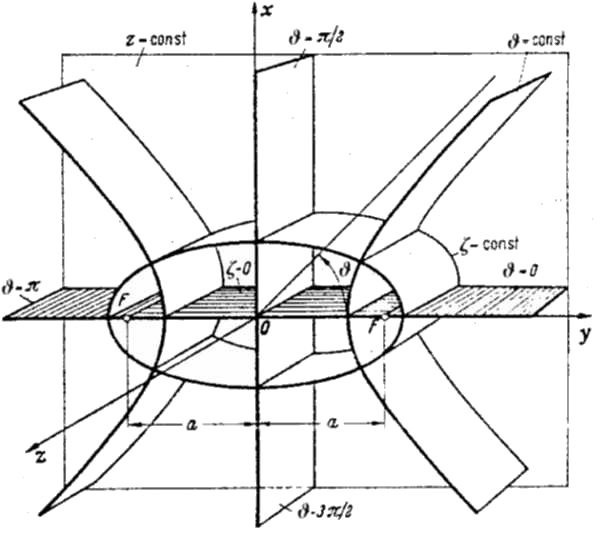
\includegraphics[scale=0.3]{Imagenes/Elliptic-cylindrical-coordinates_02.png}
    \caption{Sistema coordenado cilíndrico elíptico en una vista 3D.}
    \label{fig:figura_coordenada_cilindricas_elipticas_3D}
\end{figure}
\end{frame}

\subsection{Factores de escala}

\begin{frame}
\frametitle{Factores de escala}
Calculamos los factores de escala o coeficientes métricos a partir de la expresión:
\pause
\begin{eqnarray*}
h_{i} &=& \abs{\pdv{\vb{r}}{u_{i}}} \\[0.5em] \pause
h_{i} &=& \sqrt{ \left( \pdv{x}{u_{i}} \right)^{2} + \left( \pdv{y}{u_{i}} \right)^{2} + \left( \pdv{z}{u_{i}} \right)^{2}}
\end{eqnarray*}
\end{frame}
\begin{frame}
\frametitle{Factores de escala}
Tenemos entonces que:
\pause
\begin{align*}
x &= a \, \cosh u \, \cos v \\[0.5em]
y &= a \, \sinh u \, \sin v \\[0.5em]
z &= z \\[0.5em]
h_{1} &= h_{u} = \sqrt{ \left( \pdv{x}{u} \right)^{2} + \left( \pdv{y}{u} \right)^{2} + \left( \pdv{z}{u} \right)^{2}}
\end{align*}
\end{frame}
\begin{frame}
\frametitle{Factores de escala}
Donde las derivadas parciales son:
\pause
\begin{eqnarray*}
\begin{aligned}
\pdv{x}{u} &= a \, \sinh u \cos v \hspace{0.35cm} \Rightarrow \hspace{0.35cm} \pause \left( \pdv{x}{u} \right)^{2} = a^{2} \, \sinh^{2} u \, \cos^{2} v \\[0.5em] \pause 
\pdv{y}{u} &= a \, \cosh u \sin v \hspace{0.35cm} \Rightarrow \hspace{0.35cm} \pause \left( \pdv{y}{u} \right)^{2} = a^{2} \, \cosh^{2} u \, \sin^{2} v \\[0.5em] \pause 
\pdv{z}{u} &= 0
\end{aligned}
\end{eqnarray*}
\end{frame}
\begin{frame}
\frametitle{Factores de escala: $h_{u}$}
Al sumar los términos del radical:
\pause
\begin{align*}
h_{u} = \sqrt{a^{2} \, \sinh^{2} u \, \cos^{2} v + a^{2} \, \cosh^{2} u \, \sin^{2} v}
\end{align*}
\pause
Haciendo el álgebra respectiva y considerando que $\cosh^{2} u - \sinh^{2} = 1$, entonces tenemos que:
\end{frame}
\begin{frame}[fragile]
\frametitle{Factores de escala: $h_{u}$}
\fontsize{12}{12}\selectfont
\vspace{-1cm}
\begin{eqnarray*}
\begin{aligned}
h_{u} &= \sqrt{a^{2} \left[ \sinh^{2} u \, \cos^{2} v + \cosh^{2} u \, \sin^{2} v \right] } = \\[0.5em] \pause
&= \sqrt{a^{2} \left[ \sinh^{2} u \, \cos^{2} v + (1 + \sinh^{2} u) \, \sin^{2} v \right] } = \\[0.5em] \pause
&= \sqrt{a^{2} \left[ \sinh^{2} u \, \cos^{2} v + \sinh^{2} u \, \sin^{2} v + \sin^{2} v \right] } = \\[0.5em] \pause
&= \sqrt{a^{2} \left[ \sinh^{2} u ( \cos^{2} v + \sin^{2} v ) + \sin^{2} v \right] } = \\[0.5em] \pause
&= \sqrt{a^{2} \left[ \sinh^{2} u + \sin^{2} v  \right] }
\end{aligned}
\end{eqnarray*}
\pause
\begin{equation*}
\hspace{-4.5cm}
\boxed{ h_{u} = a \, \sqrt{ \sinh^{2} u + \sin^{2} v}}
\end{equation*}
\end{frame}
\begin{frame}
\frametitle{El siguiente factor de escala:: $h_{v}$}
Para el factor $h_{v}$ se tiene que:
\pause
\begin{align*}
h_{v} = \sqrt{ \left( \pdv{x}{v} \right)^{2} + \left( \pdv{y}{v} \right)^{2} + \left( \pdv{z}{v} \right)^{2}}
\end{align*}
\end{frame}
\begin{frame}[fragile]
\frametitle{El siguiente factor de escala: $h_{v}$}
Entonces:
\pause
\begin{eqnarray*}
\begin{aligned}
\pdv{x}{v} &= - a \, \cosh u \sin v \hspace{0.35cm} \Rightarrow \hspace{0.35cm} \pause \left( \pdv{x}{v} \right)^{2} = a^{2} \, \cosh^{2} u \, \sin^{2} v \\[0.5em] \pause
\pdv{y}{v} &= a \, \sinh u \cos v \hspace{0.35cm} \Rightarrow \hspace{0.35cm} \pause \left( \pdv{y}{v} \right)^{2} = a^{2} \, \sinh^{2} u \, \cos^{2} v \\[0.5em] \pause
\pdv{z}{v} &= 0
\end{aligned}
\end{eqnarray*}
\end{frame}
\begin{frame}[fragile]
\frametitle{El siguiente factor de escala: $h_{v}$}
Así llegamos a:
\pause
\fontsize{12}{12}\selectfont
\begin{eqnarray*}
\begin{aligned}
h_{v} &= \sqrt{a^{2} \left[ \cosh^{2} u \, \sin^{2} v + \sinh^{2} u \, \cos^{2} v \right] } \\[0.5em] \pause
&= \sqrt{a^{2} \left[ (1 + \sinh^{2} u) \, \sin^{2} v + \sinh^{2} u \, \cos^{2} v \right] } \\[0.5em] \pause
&= \sqrt{a^{2} \left[ \sinh^{2} u (\cos^{2} v +  \sin^{2} v)+ \sin^{2} v \right] } \\[0.5em] \pause
&= \sqrt{a^{2} \left[ \sinh^{2} u + \sin^{2} v  \right] }
\end{aligned}
\end{eqnarray*}
\pause
\vspace*{-0.35cm}
\begin{equation*}
\hspace{-4.5cm}
\boxed{h_{v} = a \, \sqrt{ \sinh^{2} u + \sin^{2} v}}
\end{equation*}
\end{frame}
\begin{frame}[fragile]
\frametitle{Último factor de escala: $h_{z}$}
Para el último factor de escala $h_{z}$:
\pause
\begin{align*}
h_{z} = \sqrt{ \cancelto{0}{\left( \pdv{x}{z} \right)^{2}} + \cancelto{0}{\left( \pdv{y}{z} \right)^{2}} + \cancelto{1}{\left( \pdv{z}{z} \right)^{2}}}
\end{align*}
\pause
\vspace*{-0.35cm}
\begin{equation*}
\hspace{-4.5cm}
\boxed{h_{z} = 1}
\end{equation*}
\end{frame}
\begin{frame}
\frametitle{Los tres factores de escala}
Los tres factores de escala para este sistema coordenado cilíndrico elíptico son:
\pause
\begin{align*}
h_{u} = h_{v} &= a \, \sqrt{ \sinh^{2} u + \sin^{2} v} \\[1em]
h_{z} &= 1
\end{align*}
\end{frame}

\section{Cálculo operadores diferenciales}
\frame[allowframebreaks]{\frametitle{Temas a revisar} \tableofcontents[currentsection, hideothersubsections]}
\subsection{Gradiente}

\begin{frame}
\frametitle{Cálculo del gradiente}
Ya definimos una expresión que nos permitirá calcular el gradiente sobre una función de prueba $\phi$, una vez conocidos los factores de escala del sistema coordenado de interés:
\pause
\begin{align*}
\nabla{\phi} = \nsum_{i=1}^{3} \dfrac{\vu{e_{i}}}{h_{i}} \, \pdv{\phi}{u_{i}} = \nsum_{i=1}^{3} \vu{e}_{i} \left( \nabla{\phi} \right)_{i}
\end{align*}
\end{frame}
\begin{frame}
\frametitle{Cálculo del gradiente}
Por lo que: 
\pause
\begin{align*}
\grad{\phi} &= \nsum_{i=1}^{3} \dfrac{\vu{e_{i}}}{h_{i}} \, \pdv{\phi}{u_{i}}
\end{align*}
\pause
Entonces:
\pause
\begin{align*}
\grad{\phi} &= \dfrac{\vu{e}_{u}}{h_{u}} \pdv{\phi}{u} + \dfrac{\vu{e}_{v}}{h_{v}} \pdv{\phi}{v} + \dfrac{\vu{e}_{z}}{h_{z}} \pdv{\phi}{z}
\end{align*}
\end{frame}
\begin{frame}
\frametitle{Cálculo del gradiente}
Usando los factores de escala:
\begin{align*}
\grad{\phi} &= \dfrac{1}{a \sqrt{\sinh^{2} u + \sin^{2} v}} \vu{e}_{u} \pdv{\phi}{u} + \\[0.5em]
&+ \dfrac{1}{a \sqrt{\sinh^{2} u + \sin^{2} v}} \, \vu{e}_{v} \pdv{\phi}{v} + \vu{e_{z}} \pdv{\phi}{z}
\end{align*}
\end{frame}
\begin{frame}
\frametitle{Cálculo del gradiente}
Factorizando la expresión:
\pause
\begin{align*}
\grad{\phi} = \dfrac{1}{a \sqrt{\sinh^{2} u + \sin^{2} v}} \left[ \vu{e}_{u} \pdv{\phi}{u} + \vu{e}_{v} \pdv{\phi}{v} \right] + \vu{e_{z}} \pdv{\phi}{z}
\end{align*}
Que es la expresión para el gradiente de una función escalar en el sistema coordenado cilíndrico elíptico.
\end{frame}

\subsection{Divergencia}

\begin{frame}
\frametitle{Cálculo de la divergencia}
Para un campo vectorial $\vb{B}$, habíamos llegado al resultado:
\pause
\begin{align*}
\div{\vb{B}} = \dfrac{1}{h} \, \nsum_{i=1}^{3} \pdv{u_{i}} \left( \dfrac{B_{i} \, h}{h_{i}} \right)
\end{align*}
donde $h = h_{1} h_{2} h_{3}$, así entonces:
\end{frame}
\begin{frame}
\frametitle{Cálculo de la divergencia}
\begin{align*}
\div{\vb{B}} &= \dfrac{1}{h} \left[ \pdv{u} \left( B_{u} \, h_{2} \, h_{3} \right) + \pdv{v} \left( B_{v} \, h_{1} \, h_{3} \right) + \right. \\[0.5em]
&+ \left.\pdv{z} \left( B_{z} \, h_{1} \, h_{2} \right) \right]
\end{align*}
\pause
Al realizar las respectivas operaciones y reduciendo las expresiones (tarea moral que puedes hacer), llegamos a:
\end{frame}
\begin{frame}
\frametitle{Cálculo de la divergencia}
Haciendo $h^{\prime} = \sqrt{\sinh^{2} u + \sin^{2} v}$, tenemos que:
\pause
\begin{align*}
\div{\vb{B}} &= \dfrac{1}{a \, h^{\prime}} \left[ \pdv{u} \left( h^{\prime} \, B_{u} \right) + \pdv{v} \left( h^{\prime} \, B_{v} \right) \right] + \\[0.5em]
&+ \pdv{B_{z}}{z}
\end{align*}
\end{frame}

\subsection{Cálculo del rotacional}

\begin{frame}
\frametitle{Cálculo del rotacional}
Para calcular el rotacional de un campo vectorial, ocupamos la expresión:
\pause
\begin{align*}
\curl{\vb{B}} = \dfrac{1}{h_{1} h_{2} h_{3}} \, \mdet{
h_{1} \, \vu{e}_{1} & h_{2} \, \vu{e}_{2} & h_{3} \, \vu{e}_{3} \\
\displaystyle \pdv{u_{1}} & \displaystyle \pdv{u_{2}} & \displaystyle \pdv{u_{3}} \\
B_{1} \, h_{1} & B_{2} \, h_{2} & B_{3} \, h_{3}
}
\end{align*}
\end{frame}
\begin{frame}
\frametitle{Cálculo del rotacional}
Entonces tendremos que:
\pause
\begin{align*}
\curl{\vb{B}} &= \dfrac{\vu{e}_{u}}{h_{v} h_{z}} \left[ \displaystyle \pdv{v} \left( B_{z} \, h_{z} \right) - \pdv{z} \left( B_{v} \, h_{v} \right) \right] + \\[0.5em]
&+ \dfrac{\vu{e}_{v}}{h_{z} h_{u}} \left[ \displaystyle \pdv{u_{z}} \left( B_{u} \, h_{u} \right) - \pdv{u} \left( B_{z} \, h_{z} \right) \right] + \\[0.5em]
&+ \dfrac{\vu{e}_{z}}{h_{u} h_{v}} \left[ \displaystyle \pdv{u} \left( B_{v} \, h_{v} \right) - \pdv{v} \left( B_{u} \, h_{u} \right) \right]
\end{align*}
\end{frame}
\begin{frame}
\frametitle{Cálculo del rotacional}
Calculamos las correspondientes derivadas parciales, multiplicamos los factores de escala, para luego simplificar la expresión y presentarla en términos de un determinante.
\end{frame}
\begin{frame}
\frametitle{Cálculo del rotacional}
Haciendo $h^{\prime} = \sqrt{\sinh^{2} u + \sin^{2} v}$, llegamos a:
\pause
\begin{align*}
\curl{\vb{B}} &= \dfrac{1}{h^{\prime 2}}  \, \mdet{
h^{\prime} \, \vu{e}_{u} & h^{\prime} \, \vu{e}_{v} & \vu{e}_{z} / a \\
\displaystyle \pdv{u} & \displaystyle \pdv{v} & \displaystyle \pdv{z} \\
B_{u} \, h^{\prime} & B_{v} \, h^{\prime} & B_{z} / a
}
\end{align*}
Las cuentas quedan como tarea moral!
\end{frame}

\subsection{Laplaciano}

\begin{frame}
\frametitle{Cálculo del Laplaciano}
Para una función escalar $\phi$, definimos el Laplaciano como:
\pause
\begin{align*}
\laplacian{\phi} = \dfrac{1}{h} \, \nsum_{i=1}^{3} \pdv{u_{i}} \left( \dfrac{h}{h_{i}^{2}}  \pdv{\phi}{u_{i}} \right)
\end{align*}
con $h = h_{1} h_{2} h_{3}$.
\end{frame}
\begin{frame}
\frametitle{Cálculo del Laplaciano}
Así pues, tenemos que:
\pause
\begin{align*}
\laplacian{\phi} = \dfrac{1}{a^{2} \left( \sinh^{2} u + \sin^{2} v \right)} \left[ \pdv[2]{\phi}{u} + \pdv[2]{\phi}{v} \right] + \pdv[2]{\phi}{z}
\end{align*}
\end{frame}

\section{Más sistemas coordenados}
\frame[allowframebreaks]{\frametitle{Temas a revisar} \tableofcontents[currentsection, hideothersubsections]}
\subsection{Algunos sistemas}

\begin{frame}
\frametitle{Otros sistemas coordenados}
Al comenzar el Tema 1, se mencionó que durante nuestra formación como físicos, hemos trabajado de manera natural en al menos $3$ sistemas coordenados: cartesiano, cilíndrico y esférico.
\end{frame}
\begin{frame}
\frametitle{Otros sistemas coordenados}
Sin embargo, hay que tener en cuenta que existen otros sistemas coordenados, cada uno de ellos con sus respectivas reglas de transformación.
\end{frame}
\begin{frame}
\frametitle{La metodología de trabajo}
La revisión y procedimiento que hemos hecho con el sistema de coordenadas cilíndricas elípticas, para obtener los factores de escala así como los operadores diferenciales, es la guía con la cual podemos obtener los correspondientes de estos otros sistemas.
\end{frame}
\begin{frame}
\frametitle{Elaboración de una guía}
Sería un muy buen ejercicio moral, el que obtengas esos valores y construyas una tabla.
\end{frame}
\begin{frame}
\frametitle{Elaboración de una guía}
Es cierto que puedes consultarlos en algunos textos de física matemática, pero la práctica con el trabajo a mano, nos ayuda bastante para tener presente la secuencia de pasos, además de reforzar nuestras habilidades de razonamiento matemático.
\end{frame}
\begin{frame}
\frametitle{Ejercicio a cuenta}
\textbf{Ejercicio a cuenta: } 
Para el sistema de coordenadas esferoidales prolatas $(\xi, \eta, \phi)$, cuyas reglas de transformación son:
\begin{align*}
x &= a \: \sinh \xi \: \sin \eta \: \cos \phi\\
y &= a \: \sinh \xi \: \sin \eta \: \sin \phi\\
z &= a \: \cosh \xi \: \cos \eta
\end{align*}
\end{frame}
\begin{frame}
\frametitle{Ejercicio a cuenta}
\textbf{Ejercicio a cuenta: } 
\setbeamercolor{item projected}{bg=coral,fg=black}
\setbeamertemplate{enumerate items}{%
\usebeamercolor[bg]{item projected}%
\raisebox{1.5pt}{\colorbox{bg}{\color{fg}\footnotesize\insertenumlabel}}%
}
\begin{enumerate}[<+->]
\item Describe las superficies coordenadas del sistema.
\item Calcula de manera explícita los factores de escala $(h_{\xi}, h_{\eta}, h_{\phi})$.
\item Describe los vectores unitarios $(\vu{e}_{\xi}, \vu{e}_{\eta}, \vu{e}_{\phi})$
\item Recupera los operadores diferenciales: gradiente, divergencia, rotacional y Laplaciano en este sistema coordenado.
\end{enumerate}
\end{frame}
\begin{frame}
\frametitle{Ejercicio a cuenta}
\textocolor{blue}{Nota:} aunque en una diapositiva más adelante se indica cuáles son las superficies que se generan, así como los factores de escala, deberás de realizar todo el procedimiento para la descripción de las superficies y para el cálculo de los $h_{i}$, podrás corroborar tus resultados con esos valores.
\end{frame}

\subsection{Solución de una ecuación}

\begin{frame}
\frametitle{Motivación}
En este Tema 1 que nos refiere a la física y a la geometría, es un buen punto de partida para plantear el tema de dar solución a una ecuación bajo un nuevo sistema coordenado.
\end{frame}
\begin{frame}
\frametitle{La ecuación de Helmholtz}
La ecuación de Helmholtz:
\pause
\begin{align*}
\nabla^{2} \psi + k^{2} \: \psi = 0
%\label{eq:ecuacion_02_01}
\end{align*}
es una ecuación separable.
\\
\bigskip
\pause
Es decir, podemos reexpresar esta ecuación en un sistema coordenado distinto.
\end{frame}
\begin{frame}
\frametitle{La ecuación de Helmholtz}
En particular ésta ecuación tiene el hecho de que si:
\pause
\begin{itemize}[<+->]
\item[\ding{212}] $k^{2} = 0$, se obtiene la ecuación de Laplace.
\item[\ding{212}] $k^{2} = (+) \mbox{ constante}$, se obtiene la ecuación de Helmholtz.
\item[\ding{212}] $k^{2} = (-) \mbox{ constante}$, se obtiene la ecuación de difusión (en su parte espacial).
\item[\ding{212}] $k^{2} = \mbox{ constante } \times \mbox{ energía cinética}$, se obtiene la ecuación de onda de Schrödinger.
\end{itemize}
\end{frame}
\begin{frame}
\frametitle{La ecuación de Helmholtz}
Se ha demostrado que existen once sistemas coordenados en donde la ec. de Helmholtz puede separarse. 
\\
\bigskip
\pause
Naturalmente, hay un costo que se debemos pagar por el uso de un sistema diferente al de coordenadas cartesianas.
\end{frame}
\begin{frame}
\frametitle{Contamos con los elementos necesarios}
En este punto del Tema 1, ya podemos \enquote{pagar} ese costo por el cambio de un sistema coordenado distinto, y sería también una tarea moral que logres revisar sino en todos los sistemas que mostraremos a continuación, al menos en unos $5$ sistemas.
\end{frame}
\begin{frame}
\frametitle{Indicación importante}
Cabe señalar que en algunos textos se ocupa una notación para las nuevas coordenadas con letras del alfabeto castellano: $(u, v ,w)$.
\\
\bigskip
\pause
Otros textos ocupan letras griegas: $(\xi, \eta, \chi)$.
\end{frame}
\begin{frame}
\frametitle{Notación indistinta}
Sin pérdida de generalidad, ocupar cualquiera de las notaciones indicadas representa lo mismo.
\\
\bigskip
\pause
Lo importante es trabajar con las reglas de transformación.
\end{frame}
\begin{frame}
\frametitle{Información de otros sistemas}
A continuación presentaremos las características y propiedades importantes de algunos sistemas coordenados:
\pause
\setbeamercolor{item projected}{bg=aquamarine,fg=black}
\setbeamertemplate{enumerate items}{%
\usebeamercolor[bg]{item projected}%
\raisebox{1.5pt}{\colorbox{bg}{\color{fg}\footnotesize\insertenumlabel}}%
}
\begin{enumerate}[<+->]
\item El dominio de las coordenadas.
\item Las reglas de transformación. 
\item Los factores de escala.
\item Una representación visual de las superficies.
\end{enumerate}
\end{frame}

\subsection{Otros \texorpdfstring{$11$}{11} sistemas coordenados}

% \setlength{\belowdisplayskip}{0pt}
% \setlength{\abovedisplayshortskip}{0pt}
% \setlength{\belowdisplayshortskip}{0pt}

\begin{frame}
\frametitle{1 - Coord. cilíndricas parabólicas $(u, v, z)$}
\setlength{\abovedisplayskip}{-1pt}
\fontsize{12}{12}\selectfont
\begin{minipage}[t]{0.45\textwidth}
Dominio:
\begin{align*}
u &\in (-\infty, \infty) \\
v &\in [0, \infty) \\
z &\in (-\infty, \infty)
\end{align*}
\end{minipage}
\hspace{1cm}
\pause
\begin{minipage}[t]{0.4\textwidth}
Reglas:
\begin{align*}
x &= \dfrac{1}{2}(u^{2 } -v^{2}) \\
y &= u \: v \\
z &= z
\end{align*}
\end{minipage}%
\\[0.75em]
\pause
Factores de escala:
\begin{align*}
h_{1 } &= h_{2} = \sqrt{u^{2} +v^{2}} \\
h_{3 } &= 1
\end{align*}
\end{frame}
\begin{frame}
\frametitle{Superficies coord. cilíndricas parabólicas}
\begin{figure}[H]
  \centering
  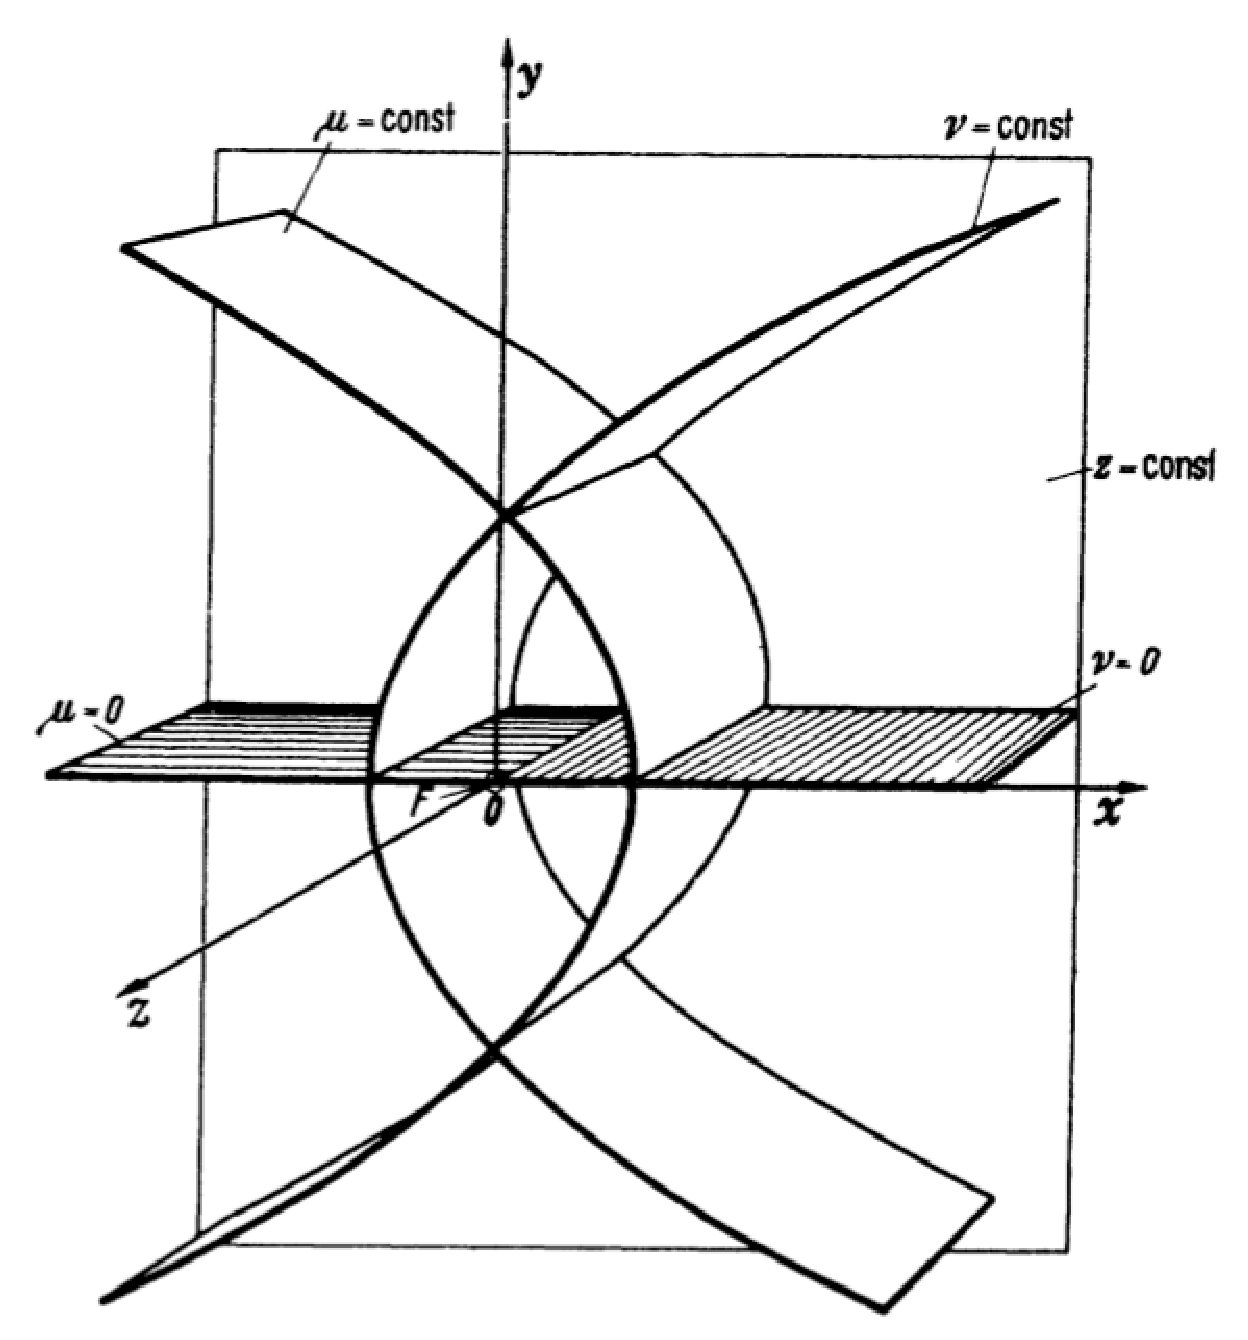
\includegraphics[scale=0.3]{Imagenes/Sistema_Cilindrico_Parabolico.eps}
\end{figure}
\end{frame}
\begin{frame}
\frametitle{2 - Coord. esferoidales prolatas $(\xi, \eta, \phi)$}
\setlength{\abovedisplayskip}{-1pt}
\fontsize{12}{12}\selectfont
\begin{minipage}[t]{0.45\textwidth}
Dominio:
\begin{align*}
\xi &\in [0, \infty) \\
\eta &\in [0, \pi] \\
\phi &\in [0, 2 \: \pi)
\end{align*}
\end{minipage}
\hspace{1cm}
\pause
\begin{minipage}[t]{0.4\textwidth}
Reglas:
\begin{align*}
x &= a \: \sinh \xi \: \sin \eta \: \cos \phi\\
y &= a \: \sinh \xi \: \sin \eta \: \sin \phi\\
z &= a \: \cosh \xi \: \cos \eta
\end{align*}
\end{minipage}%
\\[1em]
\pause
Factores de escala:
\begin{align*}
h_{1} &= h_{2} = a \: \sqrt{\sinh^{2} \xi + \sin^{2} \eta} \\
h_{3 }&= a \: \sinh \xi \: \sin \eta
\end{align*}
\end{frame}
\begin{frame}
\frametitle{Superficies coord. esferoidales prolatas}
\begin{figure}[H]
  \centering
  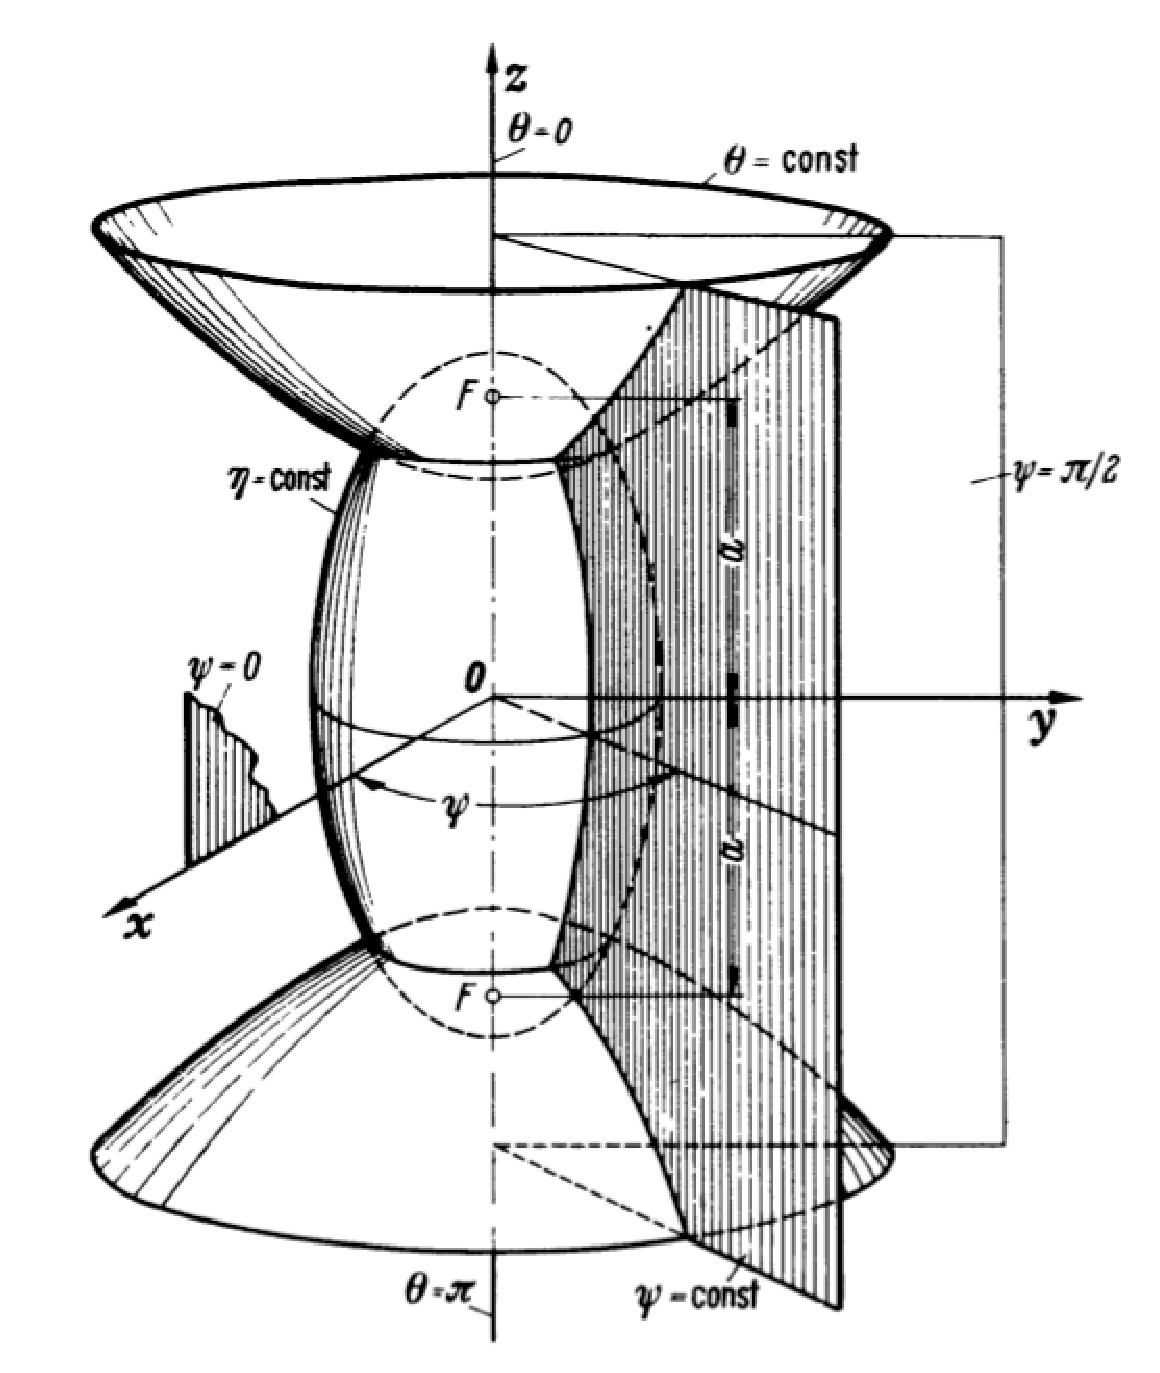
\includegraphics[scale=0.3]{Imagenes/Sistema_Esfeoridal_Prolato.eps}
\end{figure}
\end{frame}
\begin{frame}
\frametitle{3 - Coord. esferoidales oblatas $(\xi, \eta, \phi)$}
\fontsize{12}{12}\selectfont
\setlength{\abovedisplayskip}{-1pt}
\begin{minipage}{0.45\textwidth}
Dominio:
\begin{align*}
\xi &\in [0, \infty) \\
\eta &\in \left[- \dfrac{\pi}{2}, \dfrac{\pi}{2} \right] \\
\phi &\in [0, 2\: \pi)
\end{align*}
\end{minipage}
\hspace{1cm}
\pause
\begin{minipage}{0.4\textwidth}
Reglas:
\begin{align*}
x &= a \: \cosh \xi \: \cos \eta \: \cos \phi \\
y &= a \: \cosh \xi \: \cos \eta \: \sin \phi\\
z &= a \: \sinh \xi \: \sin \eta
\end{align*}
\end{minipage}%
\\[1em]
\pause
Factores de escala:
\begin{align*}
h_{1 }&= h_{2} = a \: \sqrt{\sinh^{2} \xi + \sin^{2} \eta} \\
h_{3 }&= a \: \cosh \xi \: \cos \eta
\end{align*}
\end{frame}
\begin{frame}
\frametitle{Superficies coord. esferoidales oblatas}
\begin{figure}[H]
  \centering
  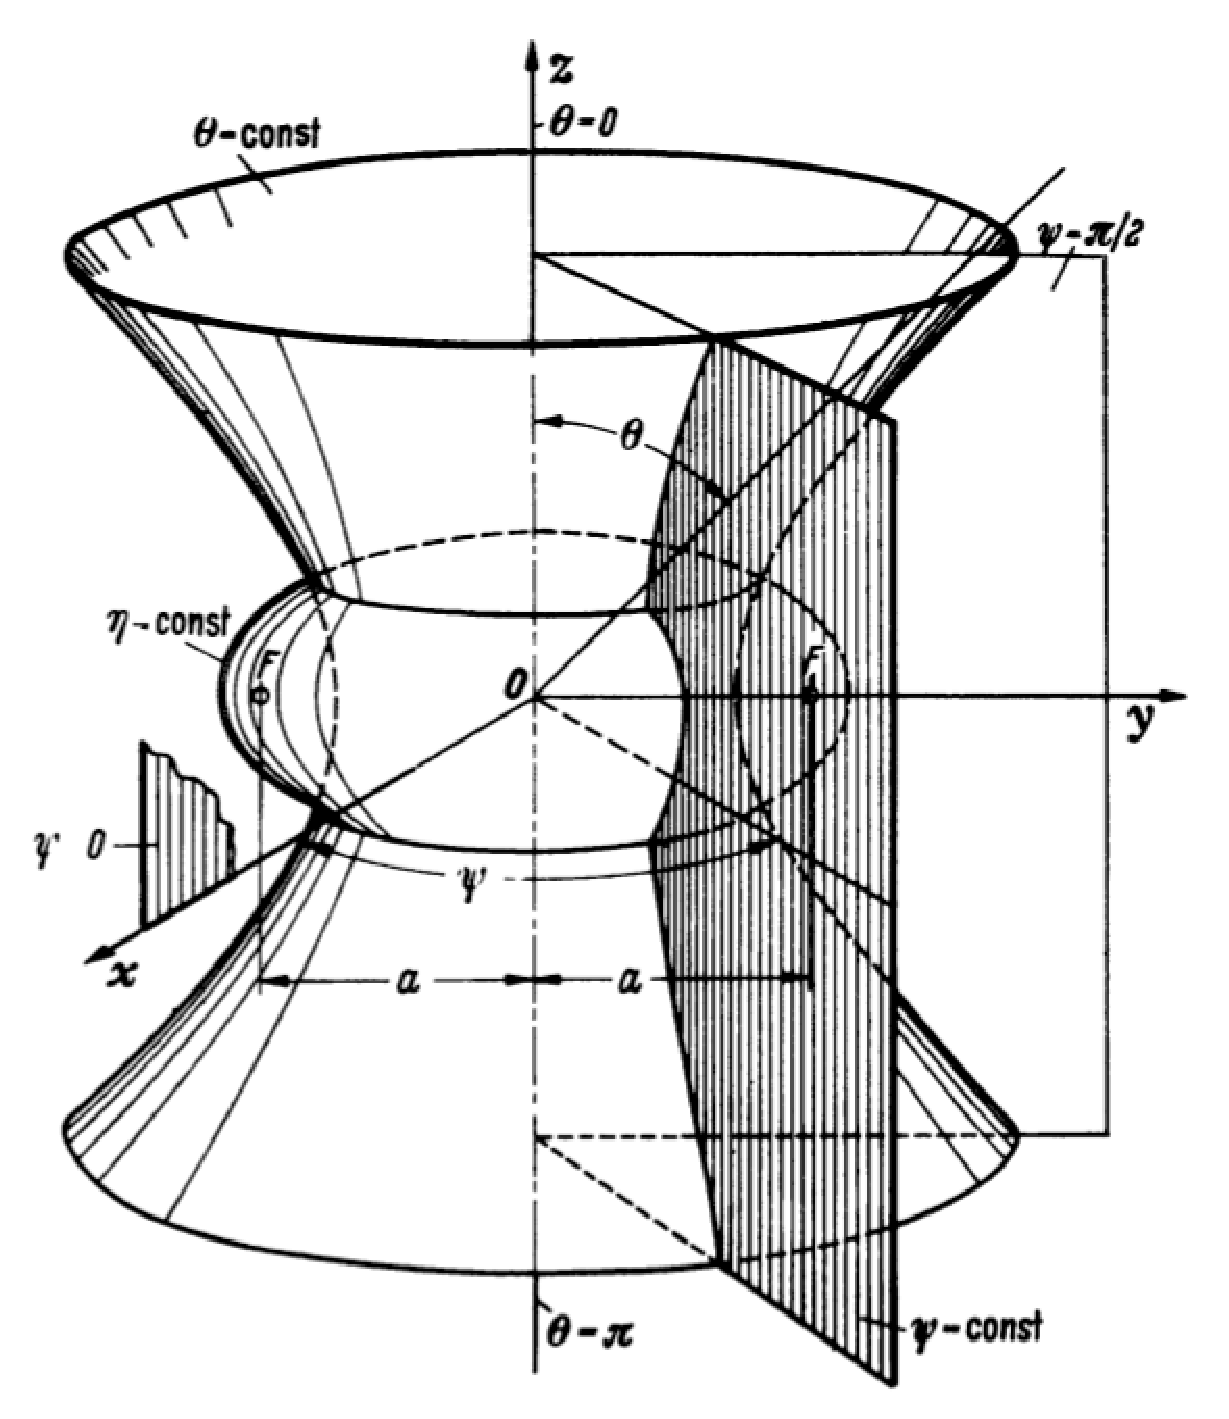
\includegraphics[scale=0.3]{Imagenes/Sistema_Esfeoridal_Oblato.eps}
\end{figure}
\end{frame}  
\begin{frame}
\frametitle{4 - Coord. parabólicas $(u, v, \phi)$}
\setlength{\abovedisplayskip}{-1pt}
\fontsize{12}{12}\selectfont
\begin{minipage}[t]{0.45\textwidth}
Dominio:
\begin{align*}
u &\in [0, \infty) \\
v &\in [0, \infty) \\
\phi &\in [0, 2 \: \pi)
\end{align*}
\end{minipage}
\hspace{1cm}
\pause
\begin{minipage}[t]{0.4\textwidth}
Reglas:
\begin{align*}
x &= u \: v \: \cos \phi \\
y &= u \: v \: \sin \phi \\
z &= \dfrac{1}{2} (u^{2} - v^{2})
\end{align*}
\end{minipage}%
\\[1em]
Factores de escala:
\begin{align*}
h_{1} &= h_{2} = \sqrt{u^{2 } +v^{2}} \\
h_{3} &= u \: v
\end{align*}
\end{frame}
\begin{frame}
\frametitle{Superficies coord. parabólicas}
\begin{figure}[H]
\centering
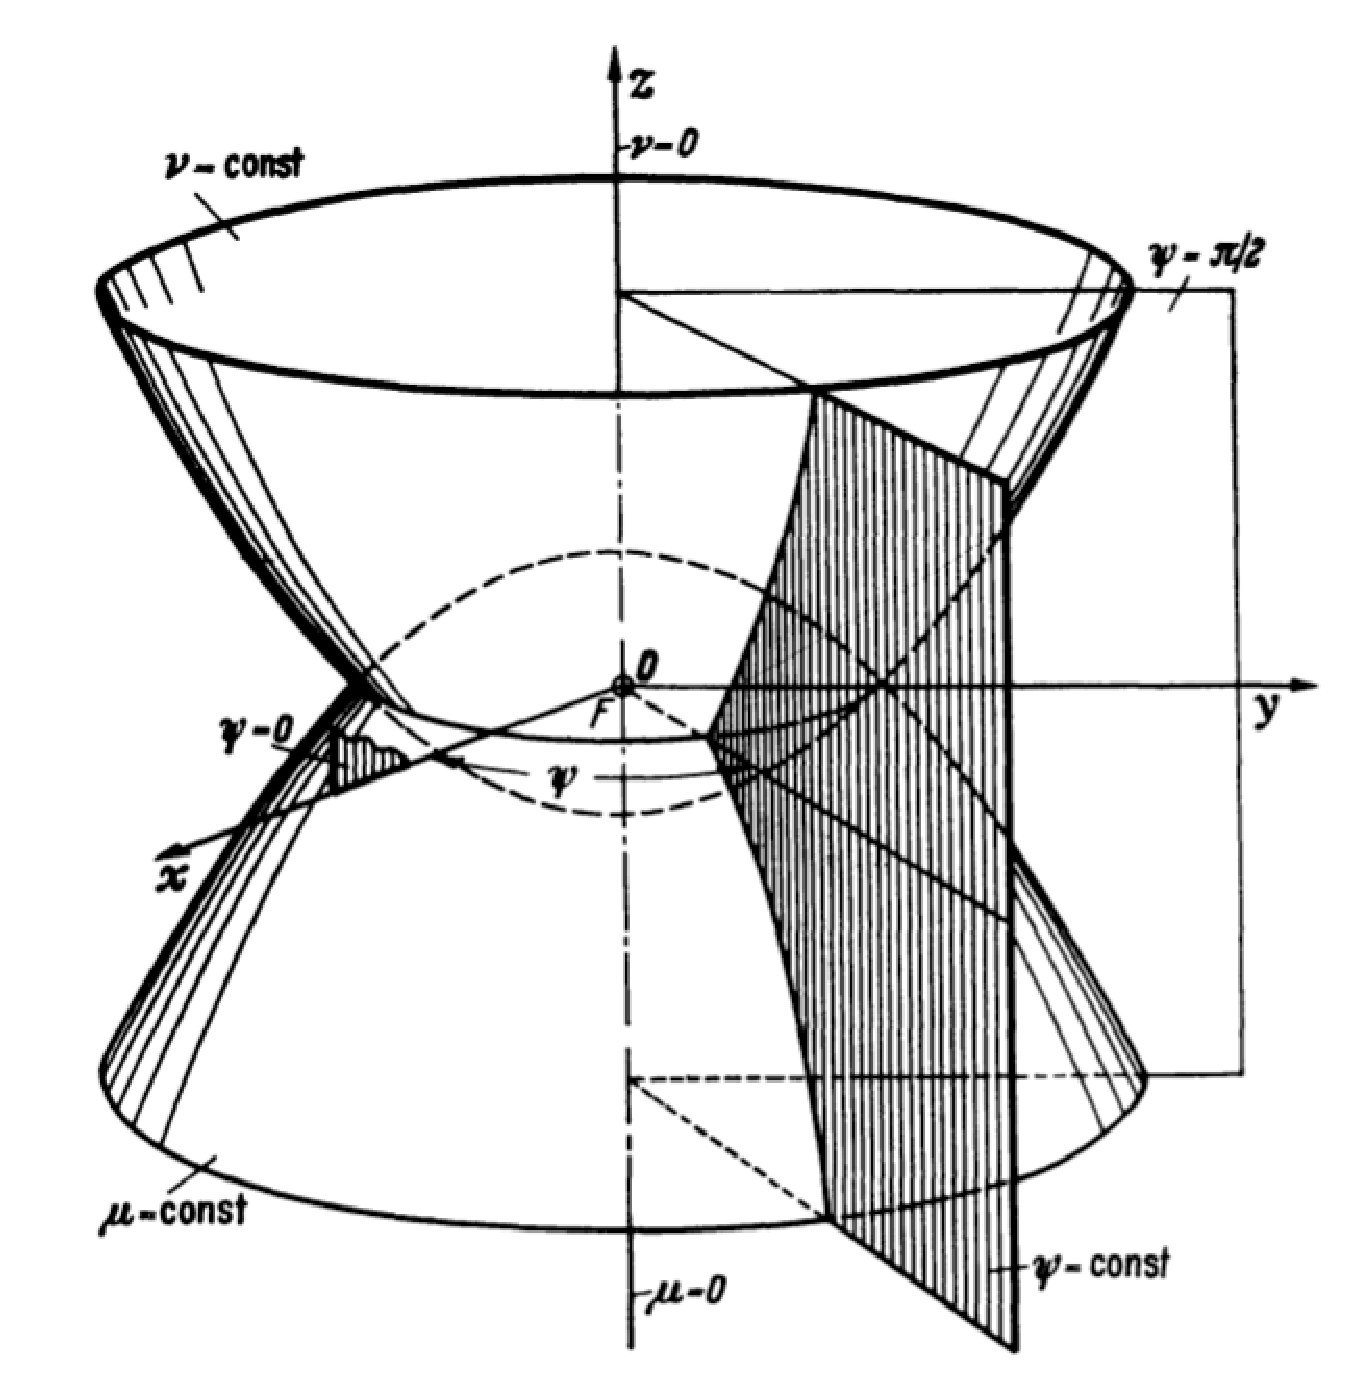
\includegraphics[scale=0.3]{Imagenes/Sistema_Parabolico.eps}
\end{figure}
\end{frame}
\begin{frame}
\frametitle{5 - Coord. cónicas $(r, \theta, \lambda)$}
\setlength{\abovedisplayskip}{-1pt}
\fontsize{12}{12}\selectfont
Dominio:
\begin{align*}
0 &\leq r < \infty \\
b^{2} &< \theta^{2} < c^{2} \\
0 &< \lambda^{2} < b^{2}
\end{align*}
Con:
\begin{align*}
c^{2} > \theta^{2} > b^{2} > \lambda^{2} > 0
\end{align*}
\end{frame}
\begin{frame}
\frametitle{5 - Coord. cónicas $(r, \theta, \lambda)$}
\setlength{\abovedisplayskip}{-1pt}
\fontsize{12}{12}\selectfont
Reglas:
\begin{align*}
(x)^{2} &= \left( \dfrac{r \, \theta \, \lambda}{b \, c} \right)^{2} \\[0.5em]
(y)^{2} &= \dfrac{r^{2} (\theta^{2} - b^{2})(b^{2} - \lambda^{2})}{b^{2}(c^{2} - b^{2})} \\[0.5em]
(z)^{2} &= \dfrac{r^{2} (c^{2} - \theta^{2})(c^{2} - \lambda^{2})}{c^{2} (c^{2} - b^{2})}
\end{align*}
\end{frame}
\begin{frame}
\frametitle{5- Coord. cónicas $(r, \theta, \lambda)$}
\setlength{\abovedisplayskip}{-1pt}
\fontsize{12}{12}\selectfont
Factores de escala:
\begin{align*}
h_{1} &= 1\\
(h_{2})^{2} &= \dfrac{r^{2} (\theta^{2} - \lambda^{2})}{(\theta^{2} - b^{2})(c^{2} - \theta^{2})} \\[0.5em]
(h_{3})^{2} &= \dfrac{r^{2} (\theta^{2} - \lambda^{2})}{(b^{2} - \lambda^{2})(c^{2} - \lambda^{2})}
\end{align*}
\end{frame}
\begin{frame}
\frametitle{Superficies coord. cónicas}
\begin{figure}[H]
\centering
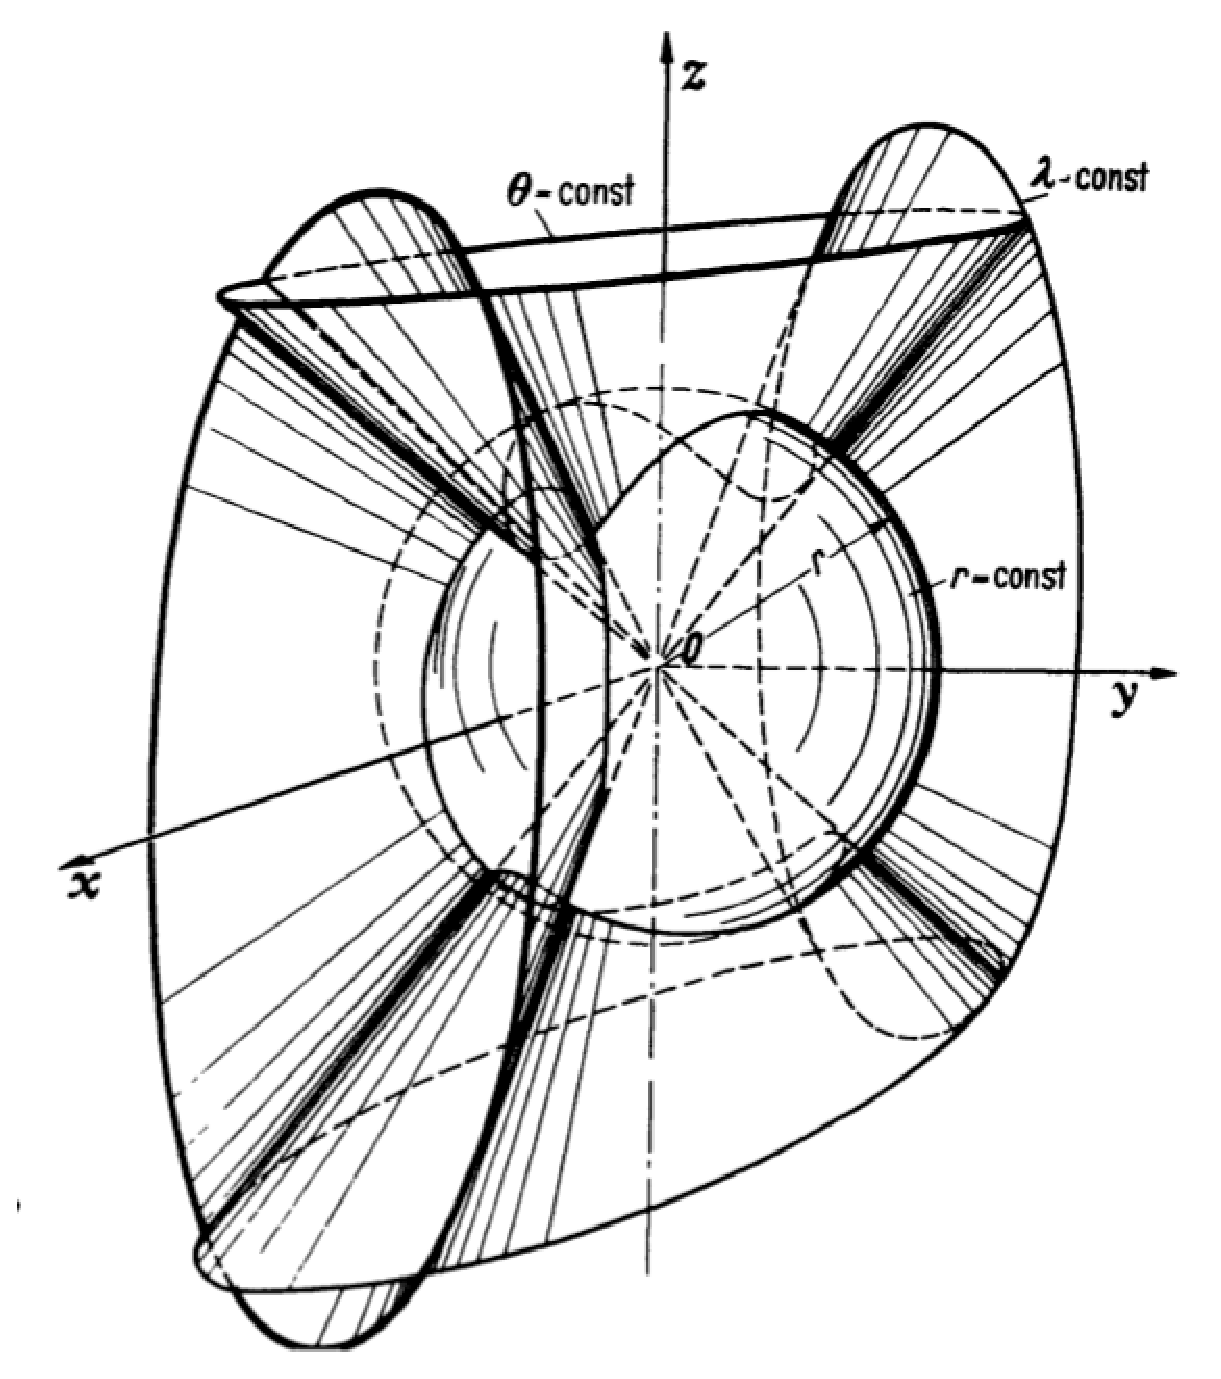
\includegraphics[scale=0.3]{Imagenes/Sistema_Conico.eps}
\end{figure}
\end{frame}

\begin{frame}
\frametitle{6 - Coord. elipsoidales $(\eta, \theta, \lambda)$}
\fontsize{12}{12}\selectfont
Dominio de las coordenadas:
\pause
\begin{align*}
c^{2} &< \eta^{2} < \infty, \\
b^{2} &< \theta^{2} < c^{2}, \\
0 &\leq \lambda^{2} < b^{2},
\end{align*}
Con
\begin{align*}
\eta^{2} > c^{2} > \theta^{2} > b^{2} > \lambda^{2} > 0
\end{align*}
\end{frame}
\begin{frame}
\frametitle{6 - Coord. elipsoidales $(\eta, \theta, \lambda)$}
\fontsize{12}{12}\selectfont
Reglas de transformación:
\pause
\begin{align*}
(x)^{2} &= \left( \dfrac{\eta \, \theta \, \lambda}{b \, c} \right)^{2} \\[0.5em]
(y)^{2} &= \dfrac{(\eta^{2} - b^{2})(\theta^{2} - b^{2})(b^{2} - \lambda^{2})}{b^{2}(c^{2} - b^{2})} \\[0.5em]
(z)^{2} &= \dfrac{(\eta^{2} - c^{2}) (c^{2} - \theta^{2})(c^{2} - \lambda^{2})}{c^{2} (c^{2} - b^{2})}
\end{align*}
\end{frame}
\begin{frame}
\frametitle{6 - Coord. elipsoidales $(\eta, \theta, \lambda)$}
\fontsize{12}{12}\selectfont
Factores de escala:
\pause
\begin{align*}
(h_{1})^{2} &= \dfrac{(\eta^{2} - \theta^{2})(\eta^{2} - \lambda^{2})}{(\eta^{2} - b^{2})(\eta^{2} - c^{2})} \\[0.5em]
(h_{2})^{2} &= \dfrac{(\theta^{2} - \lambda^{2})(\eta^{2} - \theta^{2})}{(\theta^{2} - b^{2})(c^{2} - \theta^{2})} \\[0.5em]
(h_{3})^{2} &= \dfrac{(\eta^{2} - \lambda^{2})(\theta^{2} - \lambda^{2})}{(b^{2} -  \lambda^{2})(c^{2} - \lambda^{2})}
\end{align*}
\end{frame}
\begin{frame}
\frametitle{Superficies coord. elipsoidales}
\begin{figure}[H]
\centering
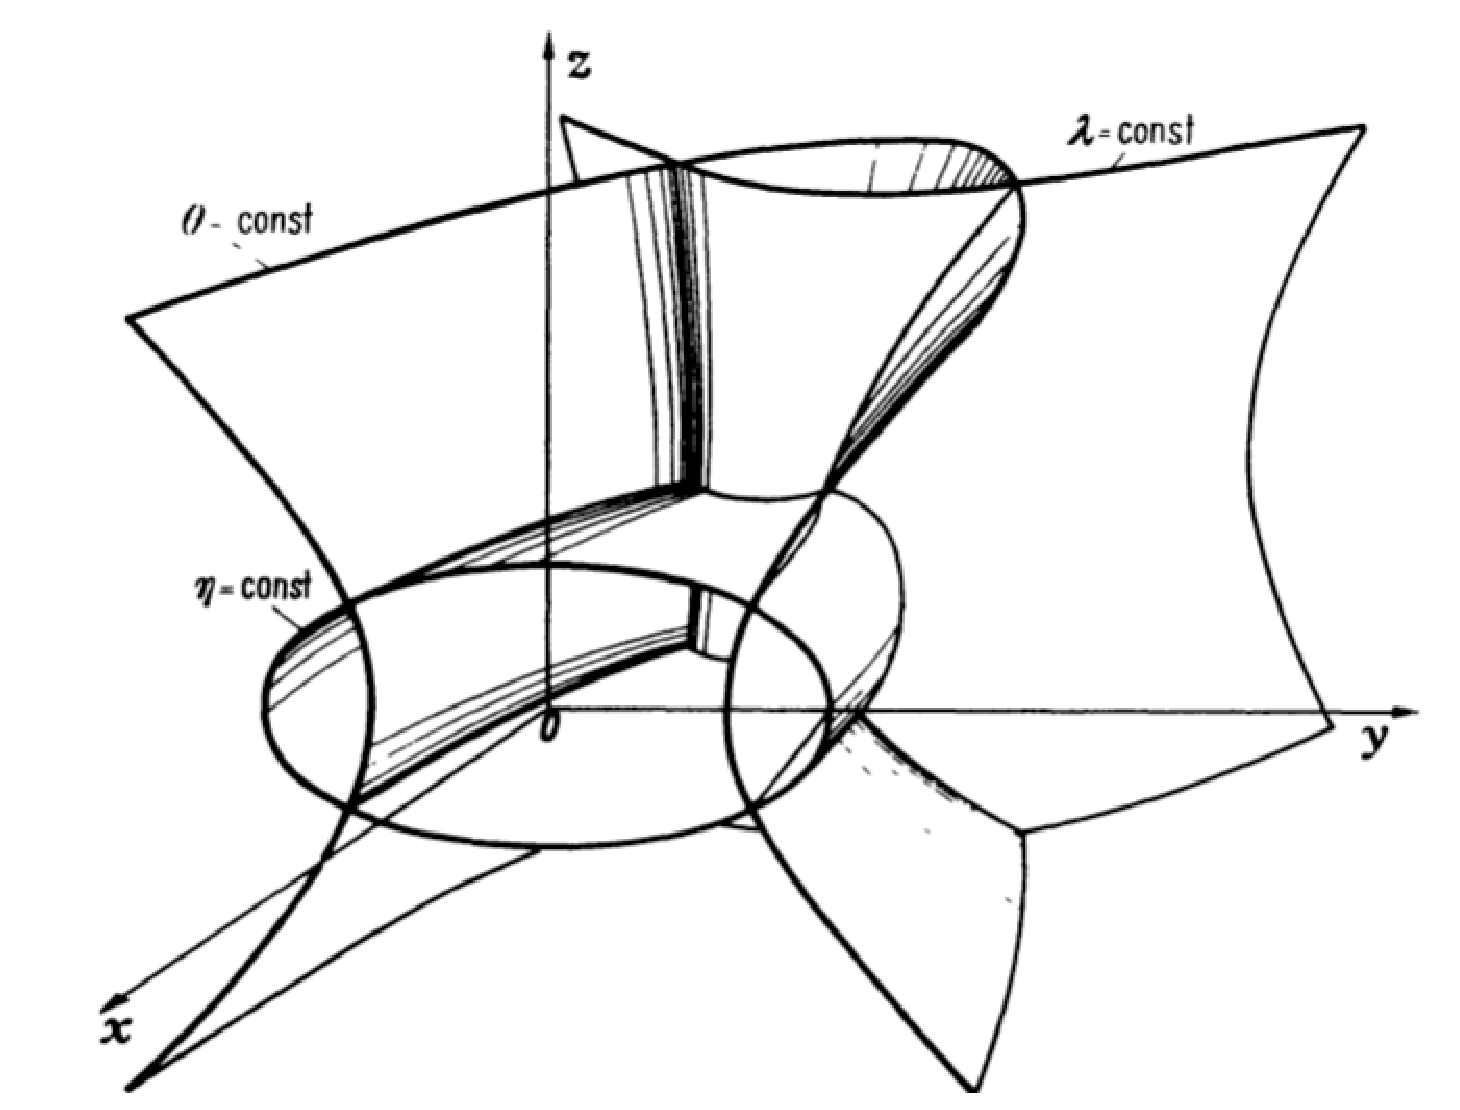
\includegraphics[scale=0.3]{Imagenes/Sistema_Elipsoidal.eps}
\end{figure}
\end{frame}

\begin{frame}
\frametitle{7 - Coord. paraboloides $(\mu, \nu, \lambda)$}
\fontsize{12}{12}\selectfont
Dominio de las coordenadas:
\pause
\begin{align*}
b &< \mu < \infty \\
0 &< \nu < c \\
c &< \lambda < b
\end{align*}
Con
\begin{align*}
\mu > b > \lambda > c > \nu > 0
\end{align*}
\end{frame}
\begin{frame}
\frametitle{7 - Coord. paraboloides $(\mu, \nu, \lambda)$}
\fontsize{12}{12}\selectfont
Reglas de transformación:
\pause
\begin{align*}
(x)^{2} &= \dfrac{4}{(b - c)} \, (\mu - b) \\[0.5em]
(y)^{2} &= \dfrac{4}{(b - c)} \, (\mu - c) \\[0.5em]
z &= \mu + \nu + \lambda - b - c
\end{align*}
\end{frame}
\begin{frame}
\frametitle{7 - Coord. paraboloides $(\mu, \nu, \lambda)$}
\fontsize{12}{12}\selectfont
Factores de escala:
\pause
\begin{align*}
(h_{1})^{2} &= \dfrac{(\mu - \nu)(\mu - \lambda)}{(\mu - b)(\mu - c)} \\[0.5em]
(h_{2})^{2} &= \dfrac{(\mu - \nu)(\lambda - \nu)}{(b - \nu)(c - \nu)} \\[0.5em]
(h_{3})^{2} &= \dfrac{(\lambda - \nu)(\mu - \lambda)}{(b - \lambda)(\lambda - c)}
\end{align*}
\end{frame}
\begin{frame}
\frametitle{Superficies coord. paraboloides}
\begin{figure}[H]
\centering
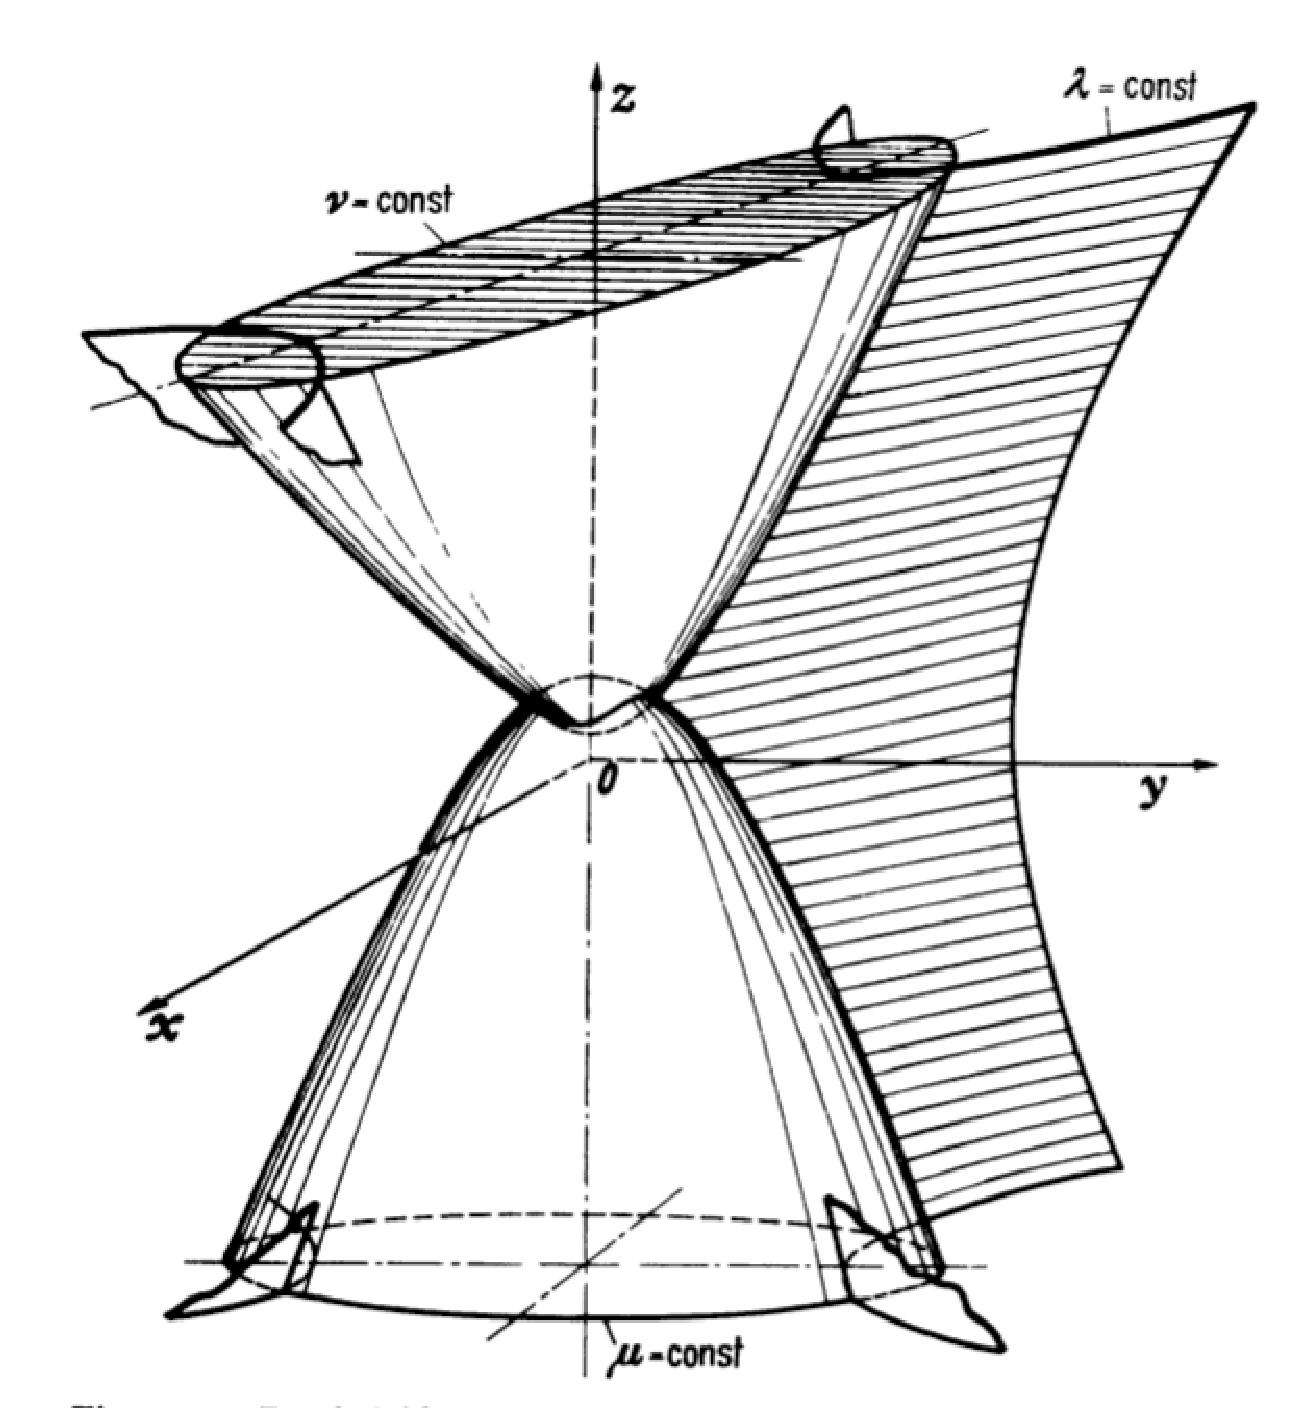
\includegraphics[scale=0.3]{Imagenes/Sistema_Paraboloide.eps}
\end{figure}
\end{frame}

\begin{frame}
\frametitle{8 - Coord. cardioide $(\mu, \nu, \psi)$}
\fontsize{12}{12}\selectfont
Dominio de las coordenadas:
\pause
\begin{align*}
0 &\leq \mu < \infty \\
0 &\leq \nu < \infty \\
0 &\leq \psi < 2 \, \pi
\end{align*}
\end{frame}
\begin{frame}
\frametitle{8 - Coord. cardioide $(\mu, \nu, \psi)$}
\fontsize{12}{12}\selectfont
Reglas de transformación:
\pause
\begin{align*}
x &= \dfrac{\mu \, \nu}{(\mu^{2} + \nu^{2})^{2}} \, \cos \psi \\[0.5em]
y &= \dfrac{\mu \, \nu}{(\mu^{2} + \nu^{2})^{2}} \, \sin \psi \\[0.5em]
z &= \dfrac{1}{2} \, \dfrac{(\mu^{2} - \nu^{2})}{(\mu^{2} + \nu^{2})^{2}}
\end{align*}
\end{frame}
\begin{frame}
\frametitle{8 - Coord. cardioide $(\mu, \nu, \psi)$}
\fontsize{12}{12}\selectfont
Factores de escala:
\pause
\begin{align*}
(h_{1})^{2} = (h_{2})^{2} &= \dfrac{1}{(\mu^{2} + \nu^{2})^{3}} \\[0.5em]
(h_{3})^{2} &= \dfrac{\mu^{2} \, \nu^{2}}{(\mu^{2} + \nu^{2})^{4}}
\end{align*}
\end{frame}
\begin{frame}
\frametitle{Superficies coord. cardioides}
\begin{figure}[H]
\centering
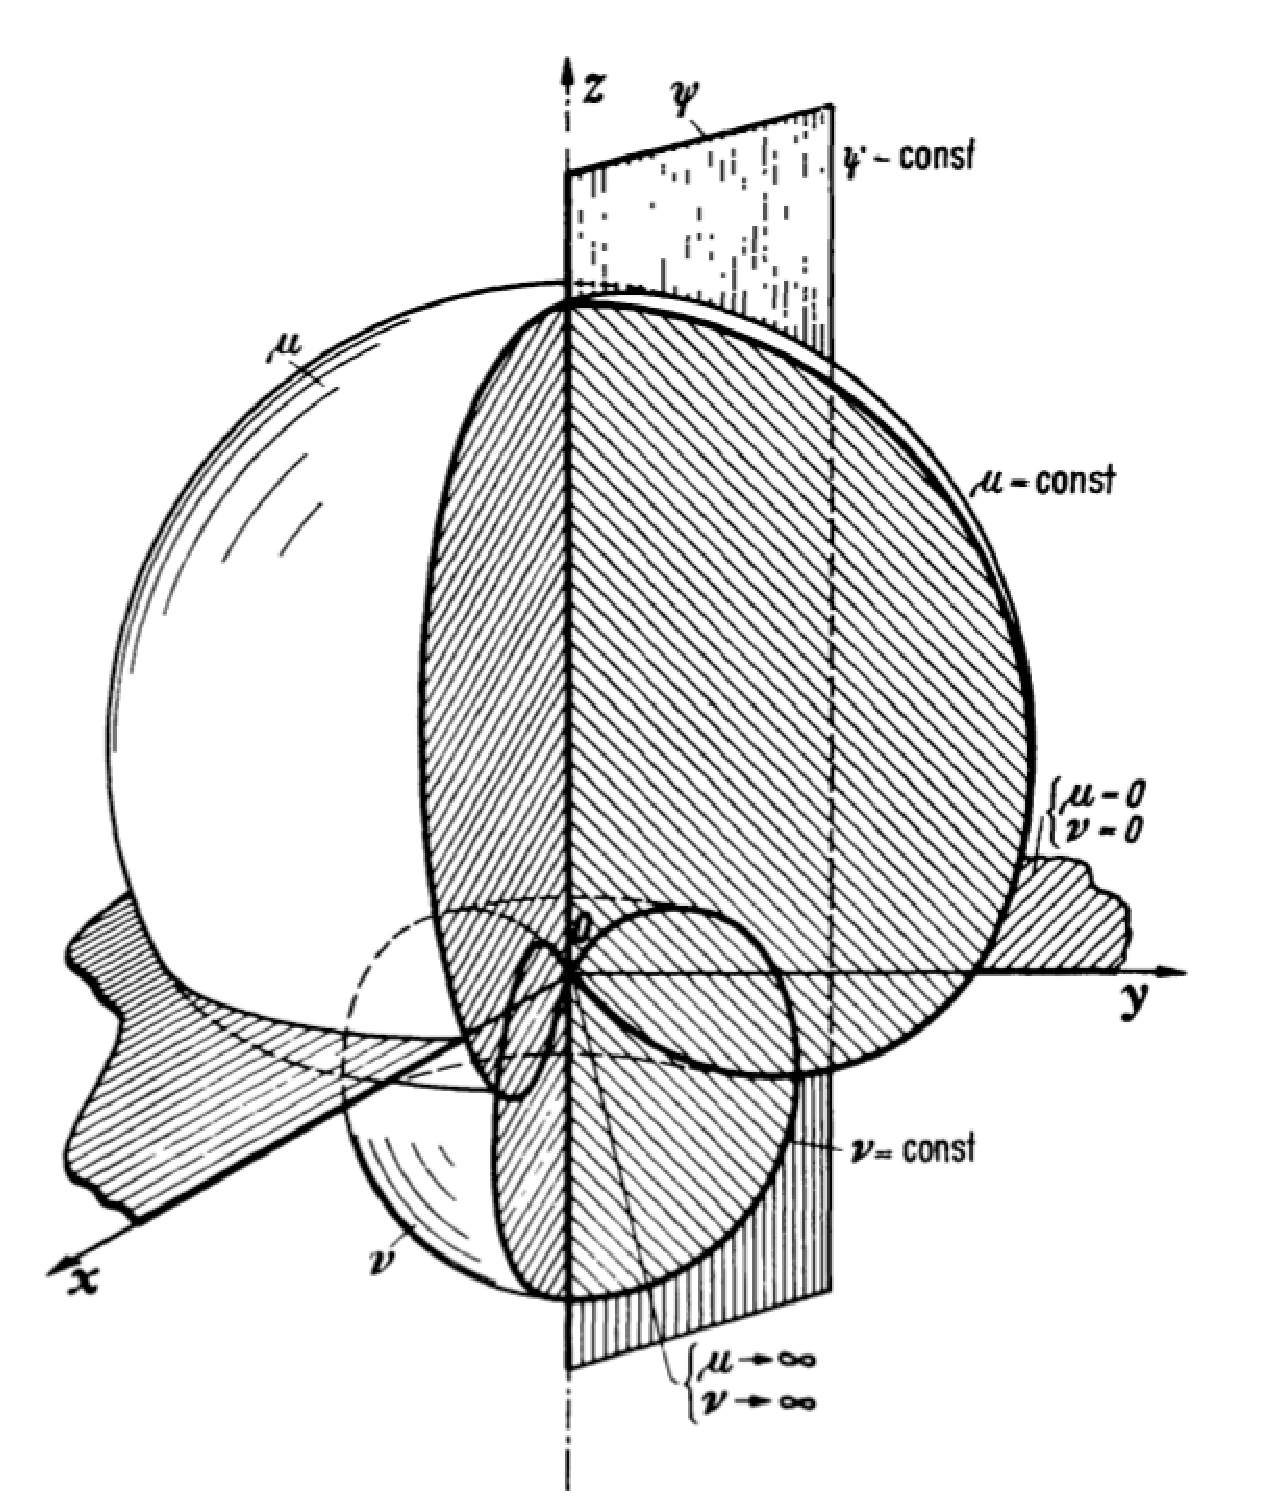
\includegraphics[scale=0.27]{Imagenes/Sistema_Cardioide.eps}
\end{figure}
\end{frame}


\begin{frame}
\frametitle{9 - Coord. biesféricas $(\eta, \theta, \psi)$}
\fontsize{12}{12}\selectfont
Dominio de las coordenadas:
\pause
\begin{align*}
-\infty &< \eta < \infty \\
0 &\leq \theta < \pi \\
0 &\leq \phi < 2\, \pi
\end{align*}
\end{frame}
\begin{frame}
\frametitle{9 - Coord. biesféricas $(\eta, \theta, \psi)$}
\fontsize{12}{12}\selectfont
Reglas de transformación:
\pause
\begin{align*}
x &= \dfrac{a \, \sin \theta \, \cos \psi}{\cosh \eta - \cos \theta} \\[0.5em]
y &= \dfrac{a \, \sin \theta \, \sin \psi}{\cosh \eta - \cos \theta} \\[0.5em]
z &= \dfrac{a \, \sinh \eta}{\cosh \eta - \cos \theta}
\end{align*}
\end{frame}
\begin{frame}
\frametitle{9 - Coord. biesféricas $(\eta, \theta, \psi)$}
\fontsize{12}{12}\selectfont
Factores de escala:
\pause
\begin{align*}
(h_{1})^{2} = (h_{2})^{2} &= \dfrac{a^{2}}{(\cosh \eta - \cos \theta)^{2}} \\[0.5em]
(h_{3})^{2} &= \dfrac{a^{2} \, \sin^{2} \theta}{(\cosh \eta - \cos \theta)^{2}}
\end{align*}
\end{frame}
\begin{frame}
\frametitle{Superficies coord. biesféricas}
\begin{figure}[H]
\centering
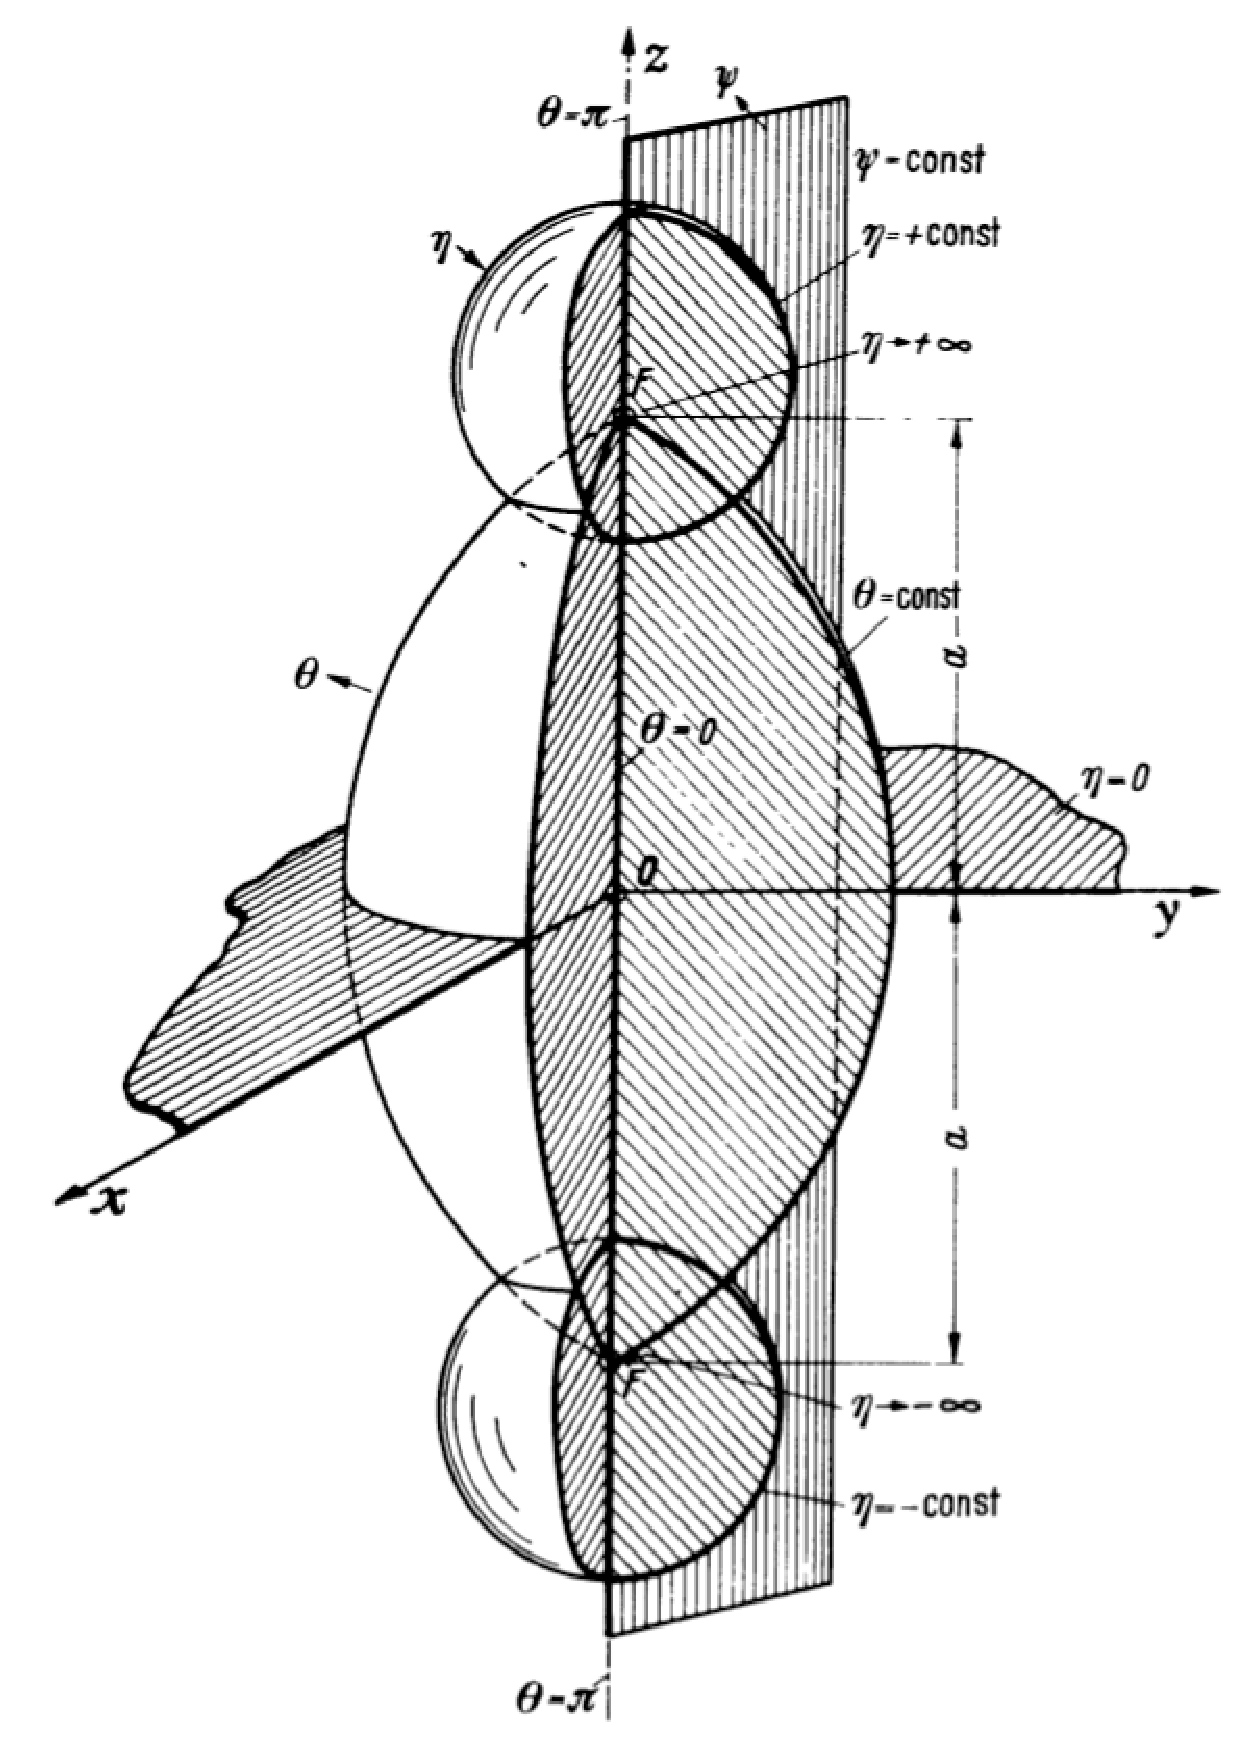
\includegraphics[scale=0.25]{Imagenes/Sistema_Biesferico.eps}
\end{figure}
\end{frame}

\begin{frame}
\frametitle{10 - Coord. toroidales $(\eta, \theta, \psi)$}
\fontsize{12}{12}\selectfont
Dominio de las coordenadas:
\pause
\begin{align*}
0 &\leq \eta < +\infty \\
-\pi &< \theta \leq +\pi \\
0 &\leq \psi < 2\, \pi
\end{align*}
\end{frame}
\begin{frame}
\frametitle{10 - Coord. toroidales $(\eta, \theta, \psi)$}
\fontsize{12}{12}\selectfont
Reglas de transformación:
\pause
\begin{align*}
x &= \dfrac{a \, \sinh \eta \, \cos \psi}{\cosh \eta - \cos \theta} \\[0.5em]
y &= \dfrac{a \, \sinh \eta \, \sin \psi}{\cosh \eta - \cos \theta} \\[0.5em]
z &= \dfrac{a \, \sin \theta}{\cosh \eta - \cos \theta}
\end{align*}
\end{frame}
\begin{frame}
\frametitle{10 - Coord. toroidales $(\eta, \theta, \psi)$}
\fontsize{12}{12}\selectfont
Factores de escala:
\pause
\begin{align*}
(h_{1})^{2} = (h_{2})^{2} &= \dfrac{a^{2}}{(\cosh \eta - \cos \theta)^{2}} \\[0.5em]
(h_{3})^{2} &= \dfrac{a^{2} \, \sinh^{2} \eta}{(\cosh \eta - \cos \theta)^{2}}
\end{align*}
\end{frame}
\begin{frame}
\frametitle{Superficies coord. toroidales}
\begin{figure}[H]
\centering
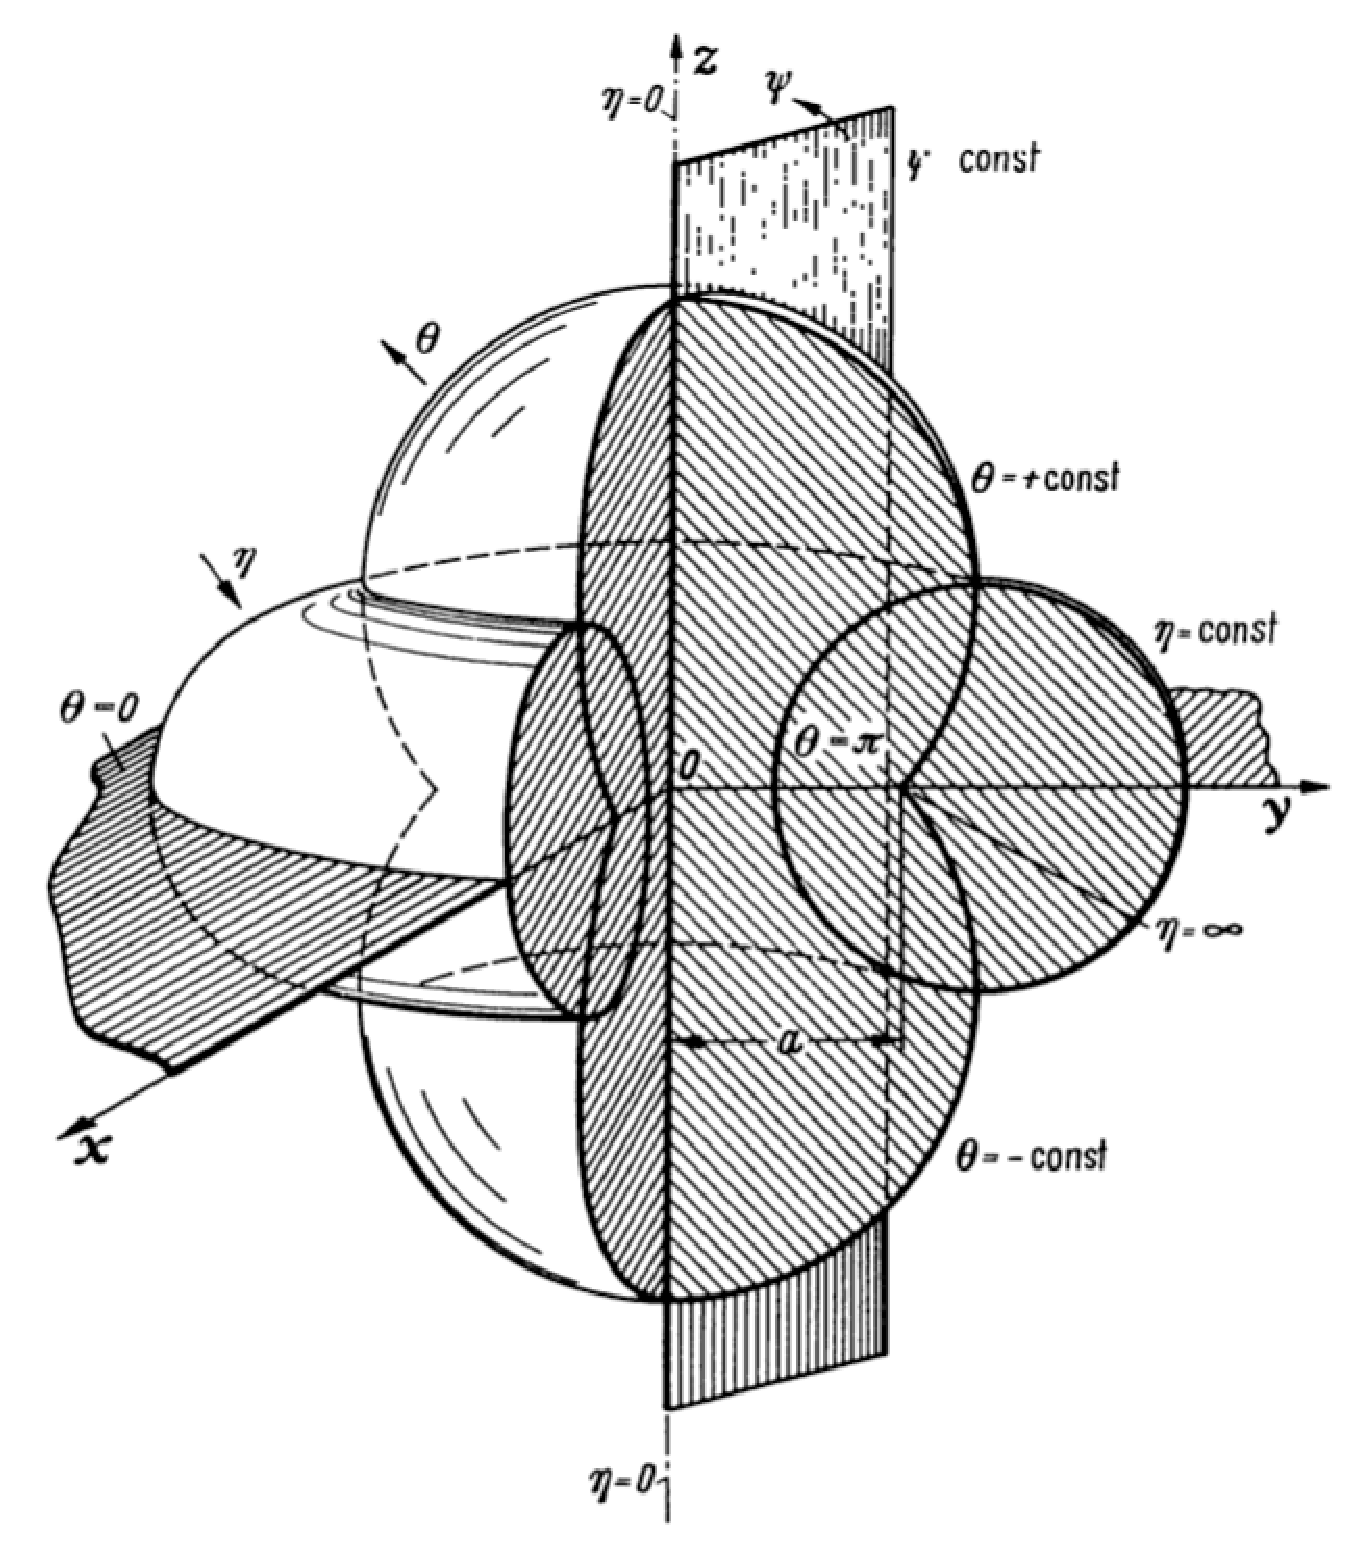
\includegraphics[scale=0.25]{Imagenes/Sistema_Toroidal.eps}
\end{figure}
\end{frame}

\section{Siguiente paso}
\frame{\frametitle{Temas a revisar} \tableofcontents[currentsection, hideothersubsections]}
\subsection{Construcción de otros sistemas}

\begin{frame}
\frametitle{El siguiente paso}
Una vez que se ha revisado la metodología para construir sistemas curvilíneos, el siguiente paso sería elaborar la descripción de las superficies coordenadas, calcular los factores de escala, obtener los elementos de línea, superficie y volumen, así como los operadores diferenciales.
\end{frame}
\begin{frame}
\frametitle{Expresión de ecuaciones diferenciales}
De esa manera ya podremos expresar la(s) ecuación(es) que definen un problema de la física bajo una geometría en particular.
\\
\bigskip
\pause
Esa tarea se desarrollará cuando se nos presente un problema específico.
\end{frame}
% \begin{frame}
% \frametitle{Ejercicio a cuenta}
% Ocupando el mismo el sistema de coordenadas esferoidales prolatas $((\xi, \eta, \phi))$ del ejercicio a cuenta anterior:
% \pause
% \setbeamercolor{item projected}{bg=bulgarianrose,fg=bubbles}
% \setbeamertemplate{enumerate items}{%
% \usebeamercolor[bg]{item projected}%
% \raisebox{1.5pt}{\colorbox{bg}{\color{fg}\footnotesize\insertenumlabel}}%
% }
% \begin{enumerate}[<+->]
% \item Calcula los operadores diferenciales $\grad{\phi}$, $\div{\vb{B}}$, $\curl{\vb{B}}$ y $\laplacian{\phi}$
% \end{enumerate}
% \end{frame}

\section{Desarrollo de un sistema coordenado 2/2}
\frame[allowframebreaks]{\frametitle{Temas a revisar} \tableofcontents[currentsection, hideothersubsections]}
\subsection{Coordenadas cónicas \texorpdfstring{$(r, \theta, \lambda)$}{(r, t, l)}.}

\begin{frame}
\frametitle{Desarrollo para un sistema especial}
A continuación veremos la manera de abordar un sistema coordenado especial, para determinar las superficies constantes, los factores de escala, los operadores diferenciales, necesarios para resolver un problema con esta geometría en particular.
\end{frame}

\subsection{Reglas de transformación}
\begin{frame}
\frametitle{Dominio de las coordenadas}
Para el sistema coordenado cónico, tenemos que:
\pause
% \begin{align*}
% y^{1} = x, \hspace{1cm} y^{2} = y, \hspace{1cm} y^{3} = z
% \end{align*}
% \pause
% junto con:
\begin{align*}
u_{1} &= r \hspace{1.5cm} 0 \leq r < \infty \\[0.35em]
u_{2} &= \theta \hspace{1.5cm} b^{2} < \theta^{2} < c^{2} \\[0.35em]
u_{3} &= \lambda \hspace{1.5cm} 0 < \lambda^{2} < b^{2}
\end{align*}
donde $c^{2} > \theta^{2} > b^{2} > \lambda^{2} > 0$
\end{frame}
\begin{frame}
\frametitle{Reglas de transformación}
Las reglas de transformación son:
\pause
\begin{align*}
x &= \dfrac{r \, \theta \, \lambda}{b \, c} \\[0.5em]
y &= \dfrac{r}{b} \, \sqrt{\dfrac{(\theta^{2} - b^{2})(\lambda^{2} - b^{2})}{(b^{2} - c^{2})}} \\[0.5em]
z &= \dfrac{r}{c} \, \sqrt{\dfrac{(\theta^{2} - c^{2})(\lambda^{2} - c^{2})}{(c^{2} - b^{2})}}
\end{align*}
\end{frame}

\subsection{Superficies coordenadas}

\begin{frame}
\frametitle{Superficies coordenadas}
Para identificar las superficies constantes, elevamos al cuadrado cada lado:
\pause
\begin{eqnarray*}
\begin{aligned}
x^{2} &= \dfrac{r^{2} \theta^{2} \lambda^{2}}{b^{2} c^{2}} \\[0.5em] \pause
y^{2} &= \dfrac{r^{2}}{b^{2}} \dfrac{(\theta^{2} - b^{2})(\lambda^{2} - b^{2})}{(b^{2} - c^{2})} \\[0.5em] \pause
z^{2} &= \dfrac{r^{2}}{c^{2}} \dfrac{(\theta^{2} - c^{2})(\lambda^{2} - c^{2})}{(c^{2} - b^{2})}
\end{aligned}
\end{eqnarray*}
\end{frame}
\begin{frame}
\frametitle{Sumando las expresiones}
Sumamos las expresiones al cuadrado:
\begin{align*}
x^{2} + y^{2} + z^{2} &= \dfrac{r^{2} \theta^{2} \lambda^{2}}{b^{2} c^{2}} + \dfrac{r^{2}}{b^{2}} \dfrac{(\theta^{2} - b^{2})(\lambda^{2} - b^{2})}{(b^{2} - c^{2})} + \\[0.5em]
&+ \dfrac{r^{2}}{c^{2}} \dfrac{(\theta^{2} - c^{2})(\lambda^{2} - c^{2})}{(c^{2} - b^{2})} =
\end{align*}
\pause
Nos armamos con paciencia para resolver la suma de fracciones, el álgebra debe de llevarse con cuidado.
\end{frame}
\begin{frame}
\frametitle{Reduciendo la expresión}\hypertarget{Suma1}
Factorizamos el término $r^{2}$:
\pause
\begin{align*}
&= r^{2} \bigg[ \dfrac{\theta^{2} \lambda^{2}}{b^{2} c^{2}} + \dfrac{1}{b^{2}} \dfrac{(\theta^{2} - b^{2})(\lambda^{2} - b^{2})}{(b^{2} - c^{2})} + \\[0.5em]
&+ \dfrac{1}{c^{2}} \dfrac{(\theta^{2} - c^{2})(\lambda^{2} - c^{2})}{(c^{2} - b^{2})} \bigg]
\end{align*}
\hyperlink{Regreso}{\beamerbutton{Regreso}}
\end{frame}
\begin{frame}
\frametitle{Analizando dos sumandos}
Nos enfocamos con los siguientes sumandos:
\pause
\begin{align*}
\dfrac{(\theta^{2} - b^{2})(\lambda^{2} - b^{2})}{b^{2}(b^{2} - c^{2})} + \dfrac{(\theta^{2} - c^{2})(\lambda^{2} - c^{2})}{c^{2}(c^{2} - b^{2})}
\end{align*}
\pause
Haciendo con cuidado el álgebra, desarrollamos cada uno de los términos:
\end{frame}
\begin{frame}
\frametitle{Desarrollando el primer término}
Entonces para el primer término:
\pause
\begin{eqnarray*}
&{}&\dfrac{(\theta^{2} - b^{2})(\lambda^{2} - b^{2})}{b^{2}(b^{2} - c^{2})} = \dfrac{\theta^{2} \lambda^{2} - \theta^2 b^{2} - \lambda^{2} b^{2} + b^{4}}{b^{2}(b^{2} - c^{2})} = \\[0.5em] \pause
&=& \dfrac{\theta^{2} \lambda^{2}}{b^{2}(b^{2} - c^{2})} - \dfrac{\theta^{2}}{(b^{2} - c^{2})} - \dfrac{\lambda^{2}}{(b^{2} - c^{2})} + \dfrac{b^{2}}{(b^{2} - c^{2})}
\end{eqnarray*}
\end{frame}
\begin{frame}
\frametitle{Desarrollando el segundo término}
Entonces para el segundo término:
\pause
\begin{eqnarray*}
&{}&\dfrac{(\theta^{2} - c^{2})(\lambda^{2} - c^{2})}{c^{2}(c^{2} - b^{2})} = \dfrac{\theta^{2} \lambda^{2} - \theta^2 c^{2} - \lambda^{2} c^{2} + c^{4}}{c^{2}(c^{2} - b^{2})} = \\[0.5em] \pause
&=& \dfrac{\theta^{2} \lambda^{2}}{c^{2}(c^{2} - b^{2})} - \dfrac{\theta^{2}}{(c^{2} - b^{2})} - \dfrac{\lambda^{2}}{(c^{2} - b^{2})} + \dfrac{c^{2}}{(c^{2} - b^{2})}
\end{eqnarray*}
\end{frame}
\begin{frame}
\frametitle{Sumando los dos términos}
Ordenando y sumando los dos términos, tendremos:
\pause
\begin{align*}
&\dfrac{\theta^{2} \lambda^{2}}{b^{2}(b^{2} - c^{2})} + \dfrac{\theta^{2} \lambda^{2}}{c^{2}(c^{2} - b^{2})} - \dfrac{\theta^{2}}{(b^{2} - c^{2})} - \dfrac{\theta^{2}}{(c^{2} - b^{2})} + \\[0.5em] 
&- \dfrac{\lambda^{2}}{(b^{2} - c^{2})} - \dfrac{\lambda^{2}}{(c^{2} - b^{2})} + \dfrac{b^{2}}{(b^{2} - c^{2})} + \dfrac{c^{2}}{(c^{2} - b^{2})}
\end{align*}
\end{frame}
\begin{frame}
\frametitle{Reduciendo los términos}
Del primero término encontrado, vemos que:
\pause
\begin{eqnarray*}
&{}&\dfrac{\theta^{2} \lambda^{2}}{b^{2}(b^{2} - c^{2})} + \dfrac{\theta^{2} \lambda^{2}}{c^{2}(c^{2} - b^{2})} = \\[0.5em] \pause
&=& \dfrac{\theta^{2} \lambda^{2} c^{2} (c^{2} - b^{2}) + \theta^{2} \lambda^{2} b^{2} (b^{2} - c^{2})}{b^{2} c^{2}(b^{2} - c^{2})(c^{2} - b^{2})} = \\[0.5em] \pause
&=& \dfrac{\theta^{2} \lambda^{2} \big[ c^{2} (c^{2} - b^{2}) + b^{2} (b^{2} - c^{2}) \big]}{b^{2} c^{2}(b^{2} - c^{2})(c^{2} - b^{2})} = \\[0.5em] \pause
&=& \dfrac{\theta^{2} \lambda^{2} (c^{4} - b^{2} c^{2} + b^{4} -b^{2} c^{2})}{-b^{2} c^{2} (b^{2} - c^{2})^{2}} = \pause - \dfrac{\theta^{2} \lambda^{2}}{b^{2} c^{2}} \Cancel[red]{\dfrac{(b^{2} - c^{2})^{2}}{(b^{2} - c^{2})^{2}}} =
\end{eqnarray*}
\end{frame}
\begin{frame}
\frametitle{Resultado reducido}
Entonces el resultado:
\pause
\begin{align*}
\dfrac{\theta^{2} \lambda^{2}}{b^{2}(b^{2} - c^{2})} + \dfrac{\theta^{2} \lambda^{2}}{c^{2}(c^{2} - b^{2})} = - \dfrac{\theta^{2} \lambda^{2}}{b^{2} c^{2}}
\end{align*}
\pause
Quedando pendientes los otros términos de la suma.
\end{frame}
\begin{frame}
\frametitle{Los otros resultados}
Es fácil revisar que:
\pause
\begin{eqnarray*}
- \dfrac{\theta^{2}}{(b^{2} {-} c^{2})} {-} \dfrac{\theta^{2}}{(c^{2} {-} b^{2})} &=& + \dfrac{\theta^{2}}{(c^{2} {-} b^{2})} {-} \dfrac{\theta^{2}}{(c^{2} {-} b^{2})} = 0 \\[0.5em] \pause
- \dfrac{\lambda^{2}}{(b^{2} {-} c^{2})} {-} \dfrac{\lambda^{2}}{(c^{2} {-} b^{2})} &=& + \dfrac{\lambda^{2}}{(c^{2} {-} b^{2})} {-} \dfrac{\lambda^{2}}{(c^{2} {-} b^{2})} = 0
\end{eqnarray*}
\end{frame}
\begin{frame}
\frametitle{Por último}
El último término que queda es:
\pause
\begin{eqnarray*}
\begin{aligned}
\dfrac{b^{2}}{(b^{2} - c^{2})} + \dfrac{c^{2}}{(c^{2} - b^{2})} &= \pause \dfrac{b^{2}}{(b^{2} - c^{2})} - \dfrac{c^{2}}{(b^{2} - c^{2})} = \\[0.5em] \pause
&= \Cancel[red]{\dfrac{(b^{2} - c^{2})}{(b^{2} - c^{2})}} = 1
\end{aligned}
\end{eqnarray*}
\end{frame}  
\begin{frame}
\frametitle{La suma completa}\hypertarget{Suma2}
Hemos llegado entonces a que la suma completa es:
\begin{eqnarray*}
x^{2} + y^{2} + z^{2} &=& \pause r^{2} \bigg[ \Cancel[blue]{\dfrac{\theta^{2} \lambda^{2}}{b^{2} c^{2}}} - \Cancel[blue]{\dfrac{\theta^{2} \lambda^{2}}{b^{2} c^{2}}} + 1 \bigg] = \\[0.5em] \pause
x^{2} + y^{2} + z^{2} &=& r^{2}
\end{eqnarray*}
\pause
Que nos definen una familia de esferas concéntricas de radio $r$, siendo la primera superficie coordenada en este sistema cónico.
\hyperlink{Regreso}{\beamerbutton{Regreso}}
\end{frame}
\begin{frame}
\frametitle{Superficie coordenada con $r$ constante}
\begin{figure}
  \centering
  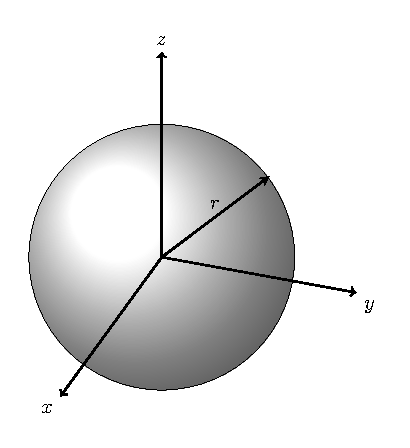
\includegraphics[scale=1]{Imagenes/Sistema_Conico_Superficie_Constante_01.eps}
\end{figure}
\end{frame}
\begin{frame}
\frametitle{Superficie coordenada con $\theta$ constante}
Al dejar que $\theta$ sea constante, y como $\theta > 0$, podemos revisar lo siguiente:
\pause
\begin{align*}
\dfrac{x^{2}}{\theta^{2}} + \dfrac{y^{2}}{\theta^{2} - b^{2}} + \dfrac{z^{2}}{\theta^{2} - c^{2}} = 0
\end{align*}
\pause
Nos define una familia de conos, que es la segunda superficie coordenada.
\end{frame}
\begin{frame}
\frametitle{Superficie coordenada con $\lambda$ constante}
Ahora hacemos que $\lambda$ sea constante, y como $\lambda > 0$, podemos revisar lo siguiente:
\pause
\begin{align*}
\dfrac{x^{2}}{\lambda^{2}} + \dfrac{y^{2}}{\lambda^{2} - b^{2}} + \dfrac{z^{2}}{\lambda^{2} - c^{2}} = 0
\end{align*}
\pause
Nos define otra familia de conos, que es la tercera superficie coordenada.
\end{frame}
\begin{frame}
\frametitle{Intersección de las superficies}
\begin{figure}
  \centering
  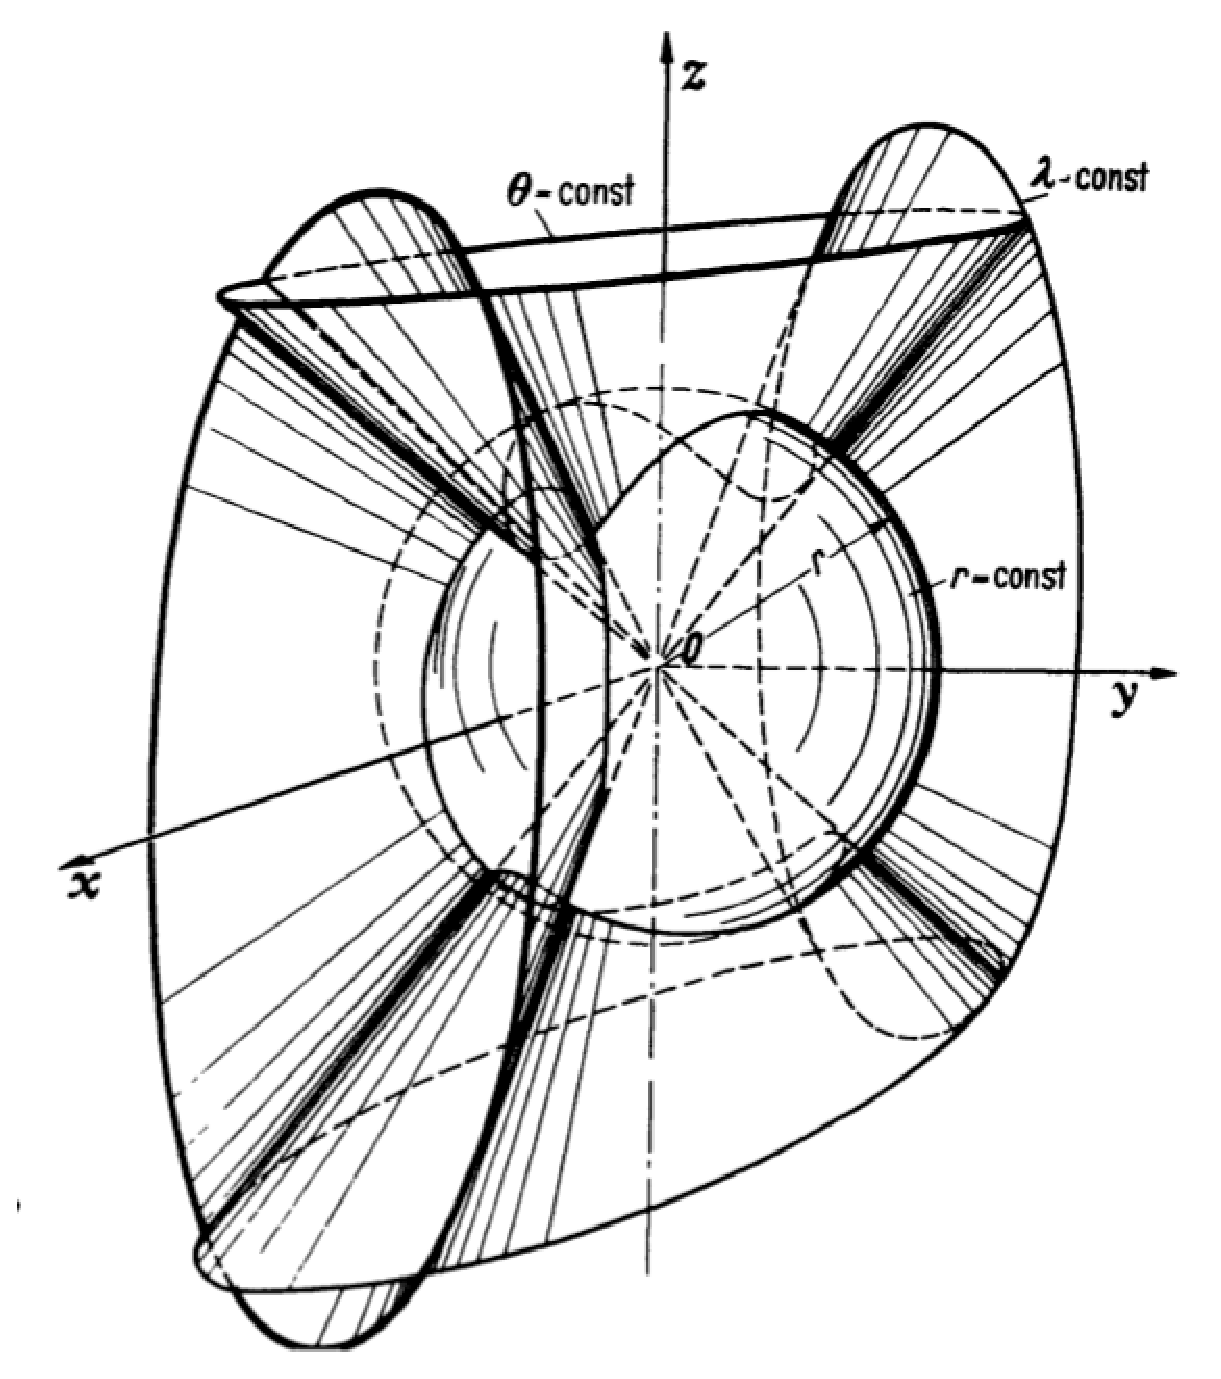
\includegraphics[scale=0.3]{Imagenes/Sistema_Conico.eps}
\end{figure}
\end{frame}

\subsection{Factores de escala}

\begin{frame}
\frametitle{Los factores de escala}
Para obtener los factores de escala, ocupamos la expresión:
\pause
\begin{eqnarray*}
h_{i} = \pause \abs{\dv{\vb{r}}{u_{i}}} = \pause \sqrt{\bigg( \pdv{x}{u_{i}} \bigg)^{2} + \bigg( \pdv{y}{u_{i}} \bigg)^{2} + \bigg( \pdv{z}{u_{i}} \bigg)^{2}}
\end{eqnarray*}
\end{frame}
\begin{frame}
\frametitle{Obteniendo $h_{r}$}
Para obtener el factor de escala $h_{r}$, debemos de calcular:
\pause
\begin{align*}
h_{r} = \sqrt{\bigg( \pdv{x}{r} \bigg)^{2} + \bigg( \pdv{y}{r} \bigg)^{2} + \bigg( \pdv{z}{r} \bigg)^{2}}
\end{align*}
\end{frame}
\begin{frame}
\frametitle{Las derivadas parciales 1}
Desarrollamos de manera explícita las derivadas parciales:
\pause
\begin{eqnarray*}
\begin{aligned}
\pdv{x}{r} &= \pause \displaystyle \pdv{r} \bigg( \dfrac{r \theta \lambda}{b c} \bigg) = \pause \dfrac{\theta \lambda}{b c} \\[0.5em] \pause
\Rightarrow \hspace{0.3cm} \bigg( \pdv{x}{r} \bigg)^{2} &= \dfrac{\theta^{2} \lambda^{2}}{b^{2} c^{2}}
\end{aligned}
\end{eqnarray*}
\end{frame}
\begin{frame}
\frametitle{Las derivadas parciales 2}
\begin{eqnarray*}
\begin{aligned}
\pdv{y}{r} &= \pause \pdv{r} \bigg( \dfrac{r}{b} \sqrt{\dfrac{ (\theta^{2} - b^{2}) (\lambda^{2} - b^{2}) }{(b^{2} - c^{2})}} \bigg) = \\[0.5em] \pause
&= \dfrac{1}{b} \sqrt{\dfrac{ (\theta^{2} - b^{2}) (\lambda^{2} - b^{2}) }{(b^{2} - c^{2})}} \\[0.5em] \pause
\Rightarrow \hspace{0.3cm} \bigg( \pdv{y}{r} \bigg)^{2} &= \dfrac{1}{b^{2}} \dfrac{ (\theta^{2} - b^{2}) (\lambda^{2} - b^{2})}{(b^{2} - c^{2})}
\end{aligned}
\end{eqnarray*}
\end{frame}
\begin{frame}
\frametitle{Las derivadas parciales 3}
\begin{eqnarray*}
\begin{aligned}
\pdv{z}{r} &= \pause \pdv{r} \bigg( \dfrac{r}{c} \sqrt{\dfrac{ (\theta^{2} - c^{2}) (\lambda^{2} - c^{2}) }{(c^{2} - b^{2})}} \bigg) = \\[0.5em] \pause
&= \dfrac{1}{c} \sqrt{\dfrac{ (\theta^{2} - c^{2}) (\lambda^{2} - c^{2}) }{(c^{2} - b^{2})}} \\[0.5em] \pause
\Rightarrow \hspace{0.3cm} \bigg( \pdv{z}{r} \bigg)^{2} &= \dfrac{1}{c^{2}} \dfrac{ (\theta^{2} - c^{2}) (\lambda^{2} - c^{2}) }{(c^{2} - b^{2})}
\end{aligned}
\end{eqnarray*}
\end{frame}
\begin{frame}
\frametitle{Haciendo la suma de las derivadas parciales}
Podemos hacer la suma:
\pause
\begin{align*}
\bigg( \pdv{x}{r} \bigg)^{2} + \bigg( \pdv{y}{r} \bigg)^{2} + \bigg( \pdv{z}{r} \bigg)^{2} =
\end{align*}
Entonces:
\pause
\begin{align*}
\dfrac{\theta^{2} \lambda^{2}}{b^{2} c^{2}} + \dfrac{1}{b^{2}} \dfrac{ (\theta^{2} - b^{2}) (\lambda^{2} - b^{2})}{(b^{2} - c^{2})} + \dfrac{1}{c^{2}} \dfrac{ (\theta^{2} - c^{2}) (\lambda^{2} - c^{2}) }{(c^{2} - b^{2})}
\end{align*}
\hypertarget{Regreso}
Esta suma ya se realizó: \hyperlink{Suma1}{\beamerbutton{Suma}} \hspace{1.5cm} \hyperlink{Suma2}{\beamerbutton{Resultado}}
\end{frame}
\begin{frame}
\frametitle{El factor de escala $h_{r}$}
Entonces tenemos que:
\pause
\begin{align*}
h_{r} &= \sqrt{\bigg( \pdv{x}{r} \bigg)^{2} + \bigg( \pdv{y}{r} \bigg)^{2} + \bigg( \pdv{z}{r} \bigg)^{2}} = \\[0.5em]
&= 1
\end{align*}
\end{frame}
\begin{frame}
\frametitle{El factor de escala $h_{\theta}$}
Ocupamos nuevamente la expresión para obtener el factor de escala $h_{\theta}$:
\pause
\begin{align*}
h_{\theta} &= \sqrt{\bigg( \pdv{x}{\theta} \bigg)^{2} + \bigg( \pdv{y}{\theta} \bigg)^{2} + \bigg( \pdv{z}{\theta} \bigg)^{2}}
\end{align*}
Recomendamos hacer el cálculo de las derivadas parciales de manera paulatina, para evitar errores.
\end{frame}
\begin{frame}
\frametitle{La derivada parcial $\pdv*{x}{\theta}$}
Comenzamos con:
\pause
\begin{eqnarray*}
\begin{aligned}
\pdv{x}{\theta} &= \pause \displaystyle \pdv{\theta} \bigg( \dfrac{r \theta \lambda}{b c} \bigg) = \pause \dfrac{r \lambda}{b c} \\[0.5em] \pause
\Rightarrow \hspace{0.3cm} \bigg( \pdv{x}{\theta} \bigg)^{2} &= \dfrac{r^{2} \lambda^{2}}{b^{2} c^{2}}
\end{aligned}
\end{eqnarray*}
\end{frame}
\begin{frame}
\frametitle{La derivada parcial $\pdv*{y}{\theta}$}
\begin{eqnarray*}
\begin{aligned}
\pdv{y}{\theta} &= \pause \pdv{\theta} \bigg( \dfrac{r}{b} \sqrt{\dfrac{ (\theta^{2} - b^{2}) (\lambda^{2} - b^{2}) }{(b^{2} - c^{2})}} \bigg) = \\[0.5em] \pause
&= \dfrac{r \theta (\lambda^{2} - b^{2})}{b (b^{2} -c^{2}) \bigg[ \dfrac{(\theta^{2} - b^{2})(\lambda^{2} - b^{2})}{(b^{2} - c^{2})} \bigg]^{\frac{1}{2}}}
\end{aligned}
\end{eqnarray*}  
\end{frame}
\begin{frame}
\frametitle{La derivada parcial $\pdv*{y}{\theta}$}
\begin{eqnarray*}
\begin{aligned}
\Rightarrow \hspace{0.3cm} \bigg( \pdv{y}{\theta} \bigg)^{2} &= \dfrac{r^{2} \theta^{2} (\lambda^{2} - b^{2})^{2}}{b^{2} (b^{2} -c^{2})^{2} \bigg[ \dfrac{(\theta^{2} - b^{2})(\lambda^{2} - b^{2})}{(b^{2} - c^{2})} \bigg]} = \\[0.5em] \pause
&= \dfrac{r^{2} \theta^{2} (\lambda^{2} - b^{2})}{b^{2} (b^{2} - c^{2}) (\theta^{2} - b^{2})}
\end{aligned}
\end{eqnarray*}  
\end{frame}
\begin{frame}
\frametitle{La derivada parcial $\pdv*{z}{\theta}$}
Para la tercera derivada parcial:
\pause
\begin{eqnarray*}
\begin{aligned}
\pdv{z}{\theta} &= \pause \pdv{\theta} \bigg( \dfrac{r}{c} \sqrt{\dfrac{(\theta^{2} - c^{2})(\lambda^{2} - c^{2})}{(c^{2} - b^{2})}} \bigg) = \\[0.5em] \pause
&= \dfrac{r \theta (\lambda^{2} - c^{2})}{c (c^{2} - b^{2}) \bigg[ \dfrac{(\theta^{2} - c^{2})(\lambda^{2} - c^{2})}{(c^{2} - b^{2})} \bigg]^{\frac{1}{2}}}
\end{aligned}
\end{eqnarray*}
\end{frame}
\begin{frame}
\frametitle{La derivada parcial $\pdv*{z}{\theta}$}
\begin{eqnarray*}
\begin{aligned}
\Rightarrow \hspace{0.3cm} \bigg( \pdv{z}{\theta} \bigg)^{2} &= \dfrac{r^{2} \theta^{2} (\lambda^{2} - c^{2})^{2}}{c^{2} (c^{2} - b^{2})^{2} \bigg[ \dfrac{(\theta^{2} - c^{2})(\lambda^{2} - c^{2})}{(c^{2} - b^{2})} \bigg]} = \\[0.5em] \pause
&= \dfrac{r^{2} \theta^{2} (\lambda^{2} - c^{2})^{2}}{c^{2} (c^{2} - b^{2}) (\theta^{2} - c^{2})}
\end{aligned}
\end{eqnarray*}
\end{frame}
\begin{frame}
\frametitle{Sumando las derivadas parciales}
Al sumar las tres derivadas parciales, se tiene que:
\pause
\begin{eqnarray*}
\begin{aligned}
h_{\theta} &= \sqrt{\bigg( \pdv{x}{\theta} \bigg)^{2} + \bigg( \pdv{y}{\theta} \bigg)^{2} + \bigg( \pdv{z}{\theta} \bigg)^{2}} = \\[0.5em] \pause
&= \dfrac{r^{2} \lambda^{2}}{b^{2} c^{2}} {+} \dfrac{r^{2} \theta^{2} (\lambda^{2} - b^{2})}{b^{2} (b^{2} - c^{2}) (\theta^{2} - b^{2})} {+} \dfrac{r^{2} \theta^{2} (\lambda^{2} - c^{2})^{2}}{c^{2} (c^{2} - b^{2}) (\theta^{2} - c^{2})}
\end{aligned}
\end{eqnarray*}
\end{frame}
\begin{frame}
\frametitle{El factor de escala $h_{\theta}$}
Luego de un cuidadoso trabajo algebraico, se llega al resultado:
\pause
\begin{align*}
h_{\theta} = r \sqrt{\dfrac{(\theta^{2} - \lambda^{2})}{(\theta^{2} - b^{2})(c^{2} - \theta^{2})}}
\end{align*}
\end{frame}
\begin{frame}
\frametitle{El factor de escala $h_{\lambda}$}
Siguiendo el mismo procedimiento, el tercer factor de escala para este sistema coordenado cónico es:
\pause
\begin{align*}
h_{\lambda} = r \sqrt{\dfrac{(\theta^{2} - \lambda^{2})}{(\lambda^{2} - b^{2})(\lambda^{2} - c^{2})}}
\end{align*}
\pause
En las soluciones de los ejercicios a cuenta y del examen, se debe de hacer todo el procedimiento de manera explícita.
\end{frame}
\begin{frame}
\frametitle{Los factores de escala}
Hemos calculado los factores de escala:
\pause
\begin{align*}
h_{r} &= 1 \\[0.5em]
h_{\theta} &=  r \, \sqrt{\dfrac{(\theta^{2} - \lambda^{2})}{(\theta^{2} - b^{2})(c^{2} - \theta^{2})}} \\[0.5em]
h_{\lambda} &= r \, \sqrt{\dfrac{(\theta^{2} - \lambda^{2})}{(\lambda^{2} - b^{2})(\lambda^{2} - c^{2})}}
\end{align*}
\end{frame}

\subsection{Diferencial de desplazamiento}
% \frame[allowframebreaks]{\tableofcontents[currentsection, hideothersubsections]}
% \subsection{Vectores unitarios en el sistema cónico}

\begin{frame}
\frametitle{Vectores unitarios}
De acuerdo con las notas de trabajo, los vectores unitarios se expresan como:
\pause
\begin{align*}
\vu{e}_{i} = \dfrac{1}{h_{i}} \, \pdv{\vb{r}}{u_{i}}
\end{align*}
\end{frame}

% \subsection{Diferencial de desplazamiento}

\begin{frame}
\frametitle{Obteniendo el diferencial}
El cuadrado de la distancia entre dos puntos está dado por:
\pause
\begin{align*}
\big( \dd{s} \big)^{2} = \big( h_{1} \dd{q_{1}} \big)^{2} + \big( h_{2} \dd{q_{2}} \big)^{2} + \big( h_{3} \dd{q_{3}} \big)^{2}
\end{align*}
\end{frame}
\begin{frame}
\frametitle{Estimado el diferencial de desplazamiento}
Una vez que se cuenta con los factores de escala, podemos expresar el diferencial de desplazamiento en el sistema coordenado cónico:
\pause
\begin{align*}
&\big( \dd{s} \big)^{2} = \big( \dd{r} \big)^{2} + \\[0.5em]
&+ r^{2} \big( \theta^{2} {-} \lambda^{2} \big) \bigg[ \dfrac{(\dd{\theta})^{2}}{(\theta^{2} {-} b^{2})(c^{2} {-} \theta^{2})} {+} \dfrac{(\dd{\lambda})^{2}}{(b^{2} {-} \lambda^{2})(c^{2} {-} \lambda^{2})} \bigg]
\end{align*}
\end{frame}
\begin{frame}
\frametitle{Obteniendo más elementos del sistema coordenado}
Los factores de escala pueden identificarse convenientemente mediante la relación:
\pause
\begin{align*}
\dd{s_{i}} = h_{i} \dd{q_{i}}
\end{align*}
para cualquier $\dd{q_{i}}$, conservando las otras $q$ constantes.
\end{frame}
\begin{frame}
\frametitle{Elementos de área y de volumen}
Con lo anterior, se pueden desarrollar los elementos de área y volumen:
\pause
\begin{eqnarray*}
\begin{aligned}
\dd{\sigma_{ij}} &= \dd{s_{i}} \dd{s_{j}} = h_{i} \, h_{j} \dd{q_{i}} \dd{q_{j}} \\[0.5em] \pause
\dd{\tau} &= \dd{s_{1}} \dd{s_{2}} \dd{s_{3}}= h_{1} \, h_{2} \, h_{3} \dd{q_{1}} \dd{q_{2}} \dd{q_{3}}
\end{aligned}
\end{eqnarray*}
\end{frame}

\subsection{Aplicación: La ecuación de Helmholtz}
% \frame[allowframebreaks]{\tableofcontents[currentsection, hideothersubsections]}
% \subsection{Construyendo la ecuación}

\begin{frame}
\frametitle{La ecuación de Helmholtz}
Sabemos que la ecuación de Helmholtz se expresa por:
\pause
\begin{align*}
\laplacian{E} + k \, E = 0
\end{align*}
donde $k$ es el número de onda, $E$ es la función escalar que es solución a la ecuación.
\\
\bigskip
\pause
Expresemos esta ecuación en el sistema coordenado cónico.
\end{frame}
\begin{frame}
\frametitle{El Laplaciano en coord. cónicas}
Ya conocemos la expresión para el Laplaciano en coordenadas generalizadas:
\begin{align*}
\laplacian{\varphi} = \dfrac{1}{h} \nsum_{i=1}^{3} \pdv{u_{i}} \bigg[ \dfrac{h}{h_{i}^{2}} \, \pdv{\varphi}{u_{i}}\bigg]
  \end{align*}
\pause
Por lo que hay que calcular algunos valores de manera anticipada.  
\end{frame}
\begin{frame}
\frametitle{Simplificando las operaciones}
Con la finalidad de simplificar las operaciones, hagamos que:
\pause
\begin{align*}
f(\theta) &= \sqrt{(\theta^{2} - b^{2})(c^{2} - \theta^{2})} \\[0.5em]
f(\lambda) &= \sqrt{(\lambda^{2} - b^{2})(c^{2} - \lambda^{2})}
\end{align*}
\end{frame}
\begin{frame}
\frametitle{Valores con los componentes métricos}
Se tiene que:
\pause
\begin{eqnarray*}
\begin{aligned}
\dfrac{1}{h} &= \left( \dfrac{r^{2} (\theta^{2} - \lambda^{2})}{f(\theta)^{2}} \cdot \dfrac{r^{2} (\theta^{2} - \lambda^{2})}{f(\lambda)^{2}} \right)^{\frac{1}{2}} = \\[0.5em] \pause
&= \dfrac{r^{2} (\theta^{2} - \lambda^{2})}{f(\theta) \, f(\lambda)}
\end{aligned}
\end{eqnarray*}
\end{frame}
\begin{frame}
\frametitle{Los otros valores}
Por lo que:
\begin{eqnarray*}
\begin{aligned}
\dfrac{h}{h_{r}} &= \pause \dfrac{\dfrac{r^{2}(\theta^{2} - \lambda^{2})}{f(\theta) \, f(\lambda)}}{1} \\[0.5em] \pause
&= \dfrac{r^{2}(\theta^{2} - \lambda^{2})}{f(\theta) \, f(\lambda)}
\end{aligned}
\end{eqnarray*}
\end{frame}
\begin{frame}
\frametitle{Los otros valores}
Del mismo modo:
\pause
\begin{eqnarray*}
\begin{aligned}
\dfrac{h}{h_{\theta}} &= \pause \dfrac{\dfrac{r^{2}(\theta^{2} - \lambda^{2})}{f(\theta) \, f(\lambda)}}{\dfrac{r^{2}(\theta^{2} - \lambda^{2})}{f(\theta)^{2}}} \\[0.5em] \pause
&= \dfrac{r^{2}(\theta^{2} - \lambda^{2}) f(\theta)^{2}}{r^{2}(\theta^{2} - \lambda^{2}) \, f(\theta) \, f(\lambda)} = \\[0.5em] \pause
&= \dfrac{f(\theta)}{f(\lambda)} 
\end{aligned}
\end{eqnarray*}
\end{frame}
\begin{frame}
\frametitle{Los otros valores}
Para el último valor:
\pause
\begin{eqnarray*}
\begin{aligned}
\dfrac{h}{h_{\lambda}} &= \pause \dfrac{\dfrac{r^{2}(\theta^{2} - \lambda^{2})}{f(\theta) \, f(\lambda)}}{\dfrac{r^{2}(\theta^{2} - \lambda^{2})}{f(\lambda)^{2}}} \\[0.5em] \pause
&= \dfrac{r^{2}(\theta^{2} - \lambda^{2}) f(\lambda)^{2}}{r^{2}(\theta^{2} - \lambda^{2}) \, f(\theta) \, f(\lambda)} = \\[0.5em] \pause
&= \dfrac{f(\lambda)}{f(\theta)} 
\end{aligned}
\end{eqnarray*}
\end{frame}
\begin{frame}
\frametitle{Expresando el Laplaciano}
El Laplaciano en coordenadas cónicas será entonces:
\pause
\begin{align*}
\laplacian{E} &= \dfrac{f(\theta) \, f(\lambda)}{r^{2} (\theta^{2} - \lambda^{2})} \bigg[ \pdv{r} \left( \dfrac{r^{2} (\theta^{2} - \lambda^{2})}{f(\theta) \, f(\lambda)} \, \pdv{E}{r} \right) + \\[0.5em]
&+ \pdv{\theta} \left( \dfrac{f(\theta)}{f(\lambda)} \, \pdv{E}{\theta} \right) + \pdv{\lambda} \left( \dfrac{f(\lambda)}{f(\theta)} \, \pdv{E}{\lambda} \right) \bigg]
\end{align*}
\pause
Que habrá que simplificar para entonces expresar la ecuación de Helmholtz.
\end{frame}
\begin{frame}
\frametitle{La ecuación de Helmholtz}
En el sistema coordenado cónico la ecuación de Helmholtz tiene la forma:
\pause
\begin{align*}
&\dfrac{1}{r^{2}} \pdv{r} \left( r^{2} \, \pdv{E}{r} \right) + \dfrac{f(\theta)}{r^{2} (\theta^{2} - \lambda^{2})} \, \pdv{\theta} \left( f(\theta) \, \pdv{E}{\theta} \right) + \\[0.5em]
&+ \dfrac{f(\lambda)}{r^{2} (\theta^{2} - \lambda^{2})} \, \pdv{\lambda} \left( f(\lambda) \, \pdv{E}{\lambda} \right) + k \, E = 0 \qed
\end{align*}
\end{frame}

\end{document}